\documentclass[12pt,a4paper,twoside]{article}
%%%%%%%%%%%%%%%%%%%%%%%%%%%%%%%%%%%%%%%%%%%%%%%%%%%%%%%%%%%%%%%%%%%%%%%%%%%
\usepackage[pdftex]{graphicx}      	%%% graphics for pdfLaTeX
\DeclareGraphicsExtensions{.pdf}   	%%% standard extension for included graphics
\usepackage{rotating}    				%%% causes an error if inserted in front of
												%%% DeclareGraphicsExtension
\usepackage{lscape}
\usepackage{amsfonts}
\usepackage{colordvi}
%\usepackage[pdftex]{thumbpdf}      %%% thumbnails for pdflatex
\usepackage[pdftex,                	%%% hyper-references for pdflatex
bookmarks=true,%                   	%%% generate bookmarks ...
bookmarksnumbered=true,%           	%%% ... with numbers
hypertexnames=false,%              	%%% needed for correct links to figures !!!
breaklinks=true,%                  	%%% break links if exceeding a single line
bookmarks=true,
bookmarksnumbered=false,
colorlinks=true,
pdfstartview=FitH,                 	%%% possible value Fit, FitB, FitH
linktocpage=true,
linkbordercolor={0 0 1}]{hyperref} 	%%% blue frames around links
%                                  	%%% pdfborder={0 0 1} is the default
\hypersetup{
pdfauthor   = {Reinhard Jansohn},
pdftitle    = {pythonOCC },
pdfsubject  = {pythonOCC },
pdfkeywords = {pythonOCC },
}
%%%%%%%%%%%%%%%%%%%%%%%%%%%%%%%%%%%%%%%%%%%%%%%%%%%%%%%%%%%%%%%%%%%%%%%%%%%
% Parts of the text may be set multi column
\usepackage{multicol}
%%%%%%%%%%%%%%%%%%%%%%%%%%%%%%%%%%%%%%%%%%%%%%%%%%%%%%%%%%%%%%%%%%%%%%%%%%%
% Caution: There are difficulties reported if subfigue is used with pdflatex 
% Search the web if problems arise
\usepackage{subfigure}
% A little bit more space between the subfigure title und the figure and the 
% annotation
\addtolength{\subfigcapskip}{0.5cm}
%%%%%%%%%%%%%%%%%%%%%%%%%%%%%%%%%%%%%%%%%%%%%%%%%%%%%%%%%%%%%%%%%%%%%%%%%%%
% Layout of titles
\usepackage{caption}
\captionsetup{format=hang,margin=10pt,font=small,labelfont=bf}
%%%%%%%%%%%%%%%%%%%%%%%%%%%%%%%%%%%%%%%%%%%%%%%%%%%%%%%%%%%%%%%%%%%%%%%%%%%
% empahsized equations
\usepackage{empheq}
%%%%%%%%%%%%%%%%%%%%%%%%%%%%%%%%%%%%%%%%%%%%%%%%%%%%%%%%%%%%%%%%%%%%%%%%%%%
% Umlauts, german stuff Degree sign and so on 
\usepackage[ansinew]{inputenc}
%%%%%%%%%%%%%%%%%%%%%%%%%%%%%%%%%%%%%%%%%%%%%%%%%%%%%%%%%%%%%%%%%%%%%%%%%%%
% Fonts
\usepackage[T1]{fontenc}
\newcommand{\changefont}[3]{
\fontfamily{#1} \fontseries{#2} \fontshape{#3} \selectfont}
%%%%%%%%%%%%%%%%%%%%%%%%%%%%%%%%%%%%%%%%%%%%%%%%%%%%%%%%%%%%%%%%%%%%%%%%%%%
%
% Length and distances
%
\unitlength1.0cm
\renewcommand{\baselinestretch}{1.15}              % distance between lines
\setlength{\parskip}{0.7ex plus 0.2ex minus 0.4ex} % distance between paragraphs
% some adaptions
\setlength{\oddsidemargin}{-0.3cm}
\setlength{\evensidemargin}{-0.3cm}
\setlength{\textwidth}{16.8cm}
\setlength{\textheight}{23.0cm}
\setlength{\topmargin}{-2.0cm}
\addtolength{\headheight}{1.0cm}
% sample
%
%\newlength{\somewidth}
%\setlength{\somewidth}{13.5cm}
%%%%%%%%%%%%%%%%%%%%%%%%%%%%%%%%%%%%%%%%%%%%%%%%%%%%%%%%%%%%%%%%%%%%%%%%%%%
% graphics for pdfLaTeX
\usepackage[pdftex]{graphicx}     
%%%%%%%%%%%%%%%%%%%%%%%%%%%%%%%%%%%%%%%%%%%%%%%%%%%%%%%%%%%%%%%%%%%%%%%%%%%
\usepackage{fancybox}      
%%%%%%%%%%%%%%%%%%%%%%%%%%%%%%%%%%%%%%%%%%%%%%%%%%%%%%%%%%%%%%%%%%%%%%%%%%%
\usepackage{color}
\definecolor{Blau}{rgb}{0.1,0.1,1.0}
\definecolor{Schwarz}{rgb}{0,0,0}
\definecolor{Grau}{rgb}{0.5,0.5,0.5}
\definecolor{DunkelGrau}{rgb}{0.15,0.15,0.15}
\definecolor{Hellbraun}{rgb}{0.5,0.25,0.0}
\definecolor{Magenta}{rgb}{1.0,0.0,1.0}
\definecolor{gray}{gray}{0.5}
\definecolor{green}{rgb}{0,0.5,0}
\definecolor{SourceHintergrund}{rgb}{1,1.0,0.95}
%
%%%%%%%%%%%%%%%%%%%%%%%%%%%%%%%%%%%%%%%%%%%%%%%%%%%%%%%%%%%%%%%%%%%%%%%%%%%
% Python sources
\usepackage{listings}
\usepackage{textcomp}
\usepackage{setspace}
\usepackage{palatino}
%
\renewcommand{\lstlistlistingname}{Code Listings}
\renewcommand{\lstlistingname}{Code Listing}

\lstnewenvironment{python}[1][]{
\lstset{
language=python,
basicstyle=\ttfamily\footnotesize\setstretch{1}, 	% print whole listing 
																	% footnotesize
stringstyle=\color{red},                    			% type for strings
showstringspaces=false,                     			% no special string spaces
alsoletter={1234567890},
otherkeywords={\ , \}, \{},
keywordstyle=\color{blue},
emph={access,and,break,class,continue,def,del,elif ,else,%
except,exec,finally,for,from,global,if,import,in,i s,%
lambda,not,or,pass,print,raise,return,try,while},
emphstyle=\color{black}\bfseries,
emph={[2]True, False, None, self},
emphstyle=[2]\color{green},
emph={[3]from, import, as},
emphstyle=[3]\color{blue},
upquote=true,
morecomment=[s]{"""}{"""},
commentstyle=\color{Hellbraun}\slshape,    			% type for comments  
emph={[4]1, 2, 3, 4, 5, 6, 7, 8, 9, 0},
emphstyle=[4]\color{blue},
literate=*{:}{{\textcolor{blue}:}}{1}%
{=}{{\textcolor{blue}=}}{1}%
{-}{{\textcolor{blue}-}}{1}%
{+}{{\textcolor{blue}+}}{1}%
{*}{{\textcolor{blue}*}}{1}%
{!}{{\textcolor{blue}!}}{1}%
{(}{{\textcolor{blue}(}}{1}%
{)}{{\textcolor{blue})}}{1}%
{[}{{\textcolor{blue}[}}{1}%
{]}{{\textcolor{blue}]}}{1}%
{<}{{\textcolor{blue}<}}{1}%
{>}{{\textcolor{blue}>}}{1},%
%framexleftmargin=1mm, framextopmargin=1mm, frame=shadowbox, rulesepcolor=\color{blue},#1
backgroundcolor=\color{SourceHintergrund}, 
framexleftmargin=1mm, framexrightmargin=1mm, framextopmargin=1mm, frame=single, framerule=1pt, rulecolor=\color{Schwarz},#1
}}{}
%%%%%%%%%%%%%%%%%%%%%%%%%%%%%%%%%%%%%%%%%%%%%%%%%%%%%%%%%%%%%%%%%%%%%%%%%%%
% numbering
\setcounter{secnumdepth}{5}
\setcounter{tocdepth}{4}
%%%%%%%%%%%%%%%%%%%%%%%%%%%%%%%%%%%%%%%%%%%%%%%%%%%%%%%%%%%%%%%%%%%%%%%%%%%
% document
%
\begin{document}
%%%%%%%%%%%%%%%%%%%%%%%%%%%%%%%%%%%%%%%%%%%%%%%%%%%%%%%%%%%%%%%%%%%%%%%%%%%
\begin{titlepage}
\begin{center}
{
\large 
Geometry Modeling And Visualisation 

\vspace*{0.3cm}
Using SciPy And pythonOCC
}

{

\vspace*{0.75cm}
Reinhard Jansohn

\vspace{0.5cm}
\today
}
\end{center}
{

\vspace*{0.75cm}
{\small
\begin{center}
{\bf Abstract}
\end{center}
The results of computations in 3D cannot be drawn easily on a two dimensional medium like paper.
As a consequence mathematical books and introductional texts dealing with that often do not offer many figures which help students gaining an imagination of the meaning of all the formulas.
The remedy is the application of a mathematical software combined with the visualization capabilities of a 3D modelling software.
Python~\cite{PYTHON_ORG} offers both maths (Scipy~\cite{SCIPY_ORG}) and visualization capabilities (pythonOCC~\cite{PYTHONOCC_ORG}). 
In addition Python may be learned in a few days.
This document shows how to visualise geometric computations performed with SciPy in pythonOCC.

For SciPy the documentation and other sources on the web provide a huge amount of information.
But how to create visualizations with the aid of pythonOCC? 
Looking for information about that will give you less extensive documents\footnote{This is only true for the actual version 0.4 of pythonOCC at time of writing.}.
This little paper may help you to get started creating visualizations utilising pythonOCC more painlessly.

After reading and trying the step by step examples you should be able to write your code simply by steeling snippets from the examples delivered with pythonOCC.

\begin{center}
{\bf Acknowledgement}
\end{center}
This little booklet would not exist without the support of Thomas Paviot. I also like to thank all developers of Open~Cascade and pythonOCC for their great work.
}
}
\end{titlepage}

%%%%%%%%%%%%%%%%%%%%%%%%%%%%%%%%%%%%%%%%%%%%%%%%%%%%%%%%%%%%%%%%%%%%%%%%%%%

%%%%%%%%%%%%%%%%%%%%%%%%%%%%%%%%%%%%%%%%%%%%%%%%%%%%%%%%%%%%%%%%%%%%%%%%%%%

%%%%%%%%%%%%%%%%%%%%%%%%%%%%%%%%%%%%%%%%%%%%%%%%%%%%%%%%%%%%%%%%%%%%%%%%%%%
\include{license}
\tableofcontents
\section{Step 1 - The frame}
\label{SectionStep1}
Our first step is to provide a frame which is used in the next steps.
This frame consists of a menu where we can hook functions to be selected and a canvas where all our drawings will be displayed.

Read and run {\tt Step1.py} (see listing~\ref{LISTING_STEP1_PY} given below)
\footnote{In the following sections only the relevant parts of the code is presented in the script.
If you are not sure how this code fits into the program please read the example code listing.}.

Figure~\ref{STEP_1_SCREEN} shows what you should get if you execute {\tt Step1.py}.
If you installed all what's needed you should see our empty pythonOCC screen.
Please study the code and the comments added.
If you have questions don't worry.
The comments in the code provide more information than needed for following this step by step course.
If you just accept the code as it is and try to figure out how to get something similar done that's fine for the moment.

It is interesting to note that there is no import of a GUI-framework like {\tt import~wx} in the code.
All the GUI stuff is found in {\tt OCC.Display.SimpleGui}.
In that module the environment is examined and the approprate GUI framework is initalized.
So if you like to know what is going on behind the scene have a look at {\tt OCC.Display.SimpleGui}\footnote{If you make use of wxPython you can also use the sample given in Appendix~\ref{Appendix_wx_PySimpleApp}. Here a sample of the appilcation of the class {wx.PySimpleApp} is given.}.

% +++++++++++++++++++++++++++++++++++++++++++++++++++++++++++++++++++++++ 
% +++ Bild: Step 1 ++++++++++++++++++++++++++++++++++++++++++++++++++++++
% +++++++++++++++++++++++++++++++++++++++++++++++++++++++++++++++++++++++ 
\begin{figure}[h]
\begin{center}
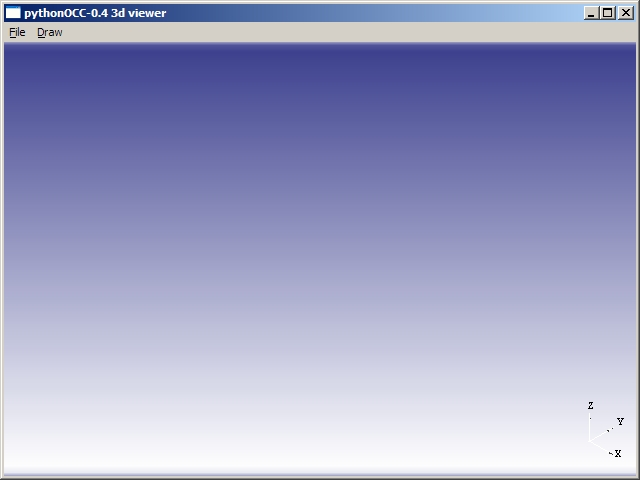
\includegraphics[height=8.5cm,width=11.3cm]{Step1.jpg}
\end{center}
\caption[Screenshot of Step1]{\label{STEP_1_SCREEN}Screenshot of Step1}
\end{figure}

\pagebreak
\begin{python}[moreemph={[4], 46, 48},caption={Step1.py - The program frame},label=LISTING_STEP1_PY]
# =============================================================================
# Packages to import
# =============================================================================
import OCC.Display.SimpleGui 
import sys
# =============================================================================
# Functions called from some menu-items
# =============================================================================
def draw_nothing(event=None):
    pass

def exit(event=None):
    sys.exit()
# =============================================================================
# Main-part: If this script is running as a main script, i.e. it 
# is directly called by Python the following is executed.
# =============================================================================
if __name__ == '__main__':
    # OCC.Display.SimpleGuiinit_display() returns multiple
    # values which are assigned here
    display, start_display, add_menu, add_function_to_menu = \
        OCC.Display.SimpleGui.init_display()
    # This is the place where we hook our functionality to menus
    # ----------------------------------------------------------
    add_menu('File')
    add_function_to_menu('File',  exit)
    add_menu('Draw')
    add_function_to_menu('Draw', draw_nothing)
    
    start_display()
\end{python}

That's the frame so get ready to add some geometry.

\section{Step 2 - Drawing Spheres}
\subsection{Drawing spheres from points}
Our first sample which adds some geometric objects is pretty simple.
Execute {\tt Step2\_1.py}, click on menu {\tt Draw} menu-item  {\tt draw sphere 1} and after that click on menu {\tt Draw} menu-item  {\tt draw sphere 2} to see the screen shown in figure~\ref{STEP_2_1_SCREEN}.
If you click on menu {\tt Erase} menu-item  {\tt erase all} the whole canvas will be erased.
% +++++++++++++++++++++++++++++++++++++++++++++++++++++++++++++++++++++++ 
% +++ Bild: Step 2_1 ++++++++++++++++++++++++++++++++++++++++++++++++++++
% +++++++++++++++++++++++++++++++++++++++++++++++++++++++++++++++++++++++ 
\begin{figure}[h]
\begin{center}
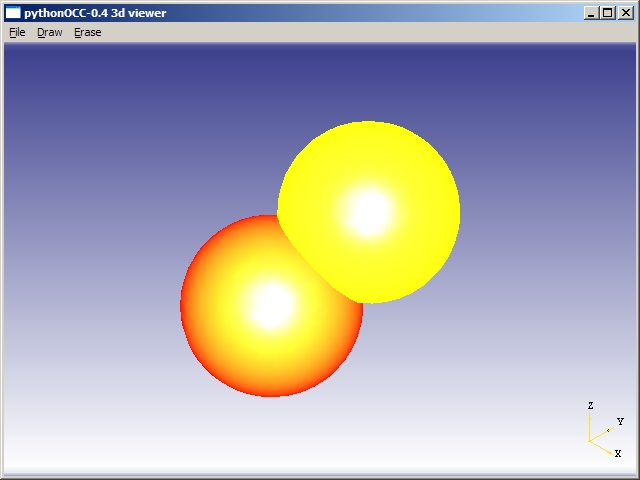
\includegraphics[height=8.5cm,width=11.3cm]{Step2_1.jpg}
\end{center}
\caption[Screenshot of Step2\_1]{\label{STEP_2_1_SCREEN}Screenshot of Step2\_1}
\end{figure}

Time to learn navigating with the mouse!
Display both spheres utilising the menu.
Do the following:
\begin{enumerate}
\item Move the mouse into the screen, press the left mouse button and hold it
		down.
		Move the mouse with the left mouse button pressed down.
		See that the coordinate system in the right corner at the bottom and the
		objects turn according to your mouse moves.
		So moving the mouse with the left mouse button held down rotates the 
		model.
		This cannot be seen with one sphere because a sphere looks the same from
		every side. 
\item Press the middle mouse button and move the mouse. 
		This causes a translation of the spheres.
\item Hold down the right mouse button and move the mouse to the left.
		The objects moves away from you.
		Now move the mouse to the right with the right mouse button held down.
		The objects come closer.
\end{enumerate}

Let's have a look at the code.
Listing~\ref{LISTING_STEP2_1_PY_A} shows how the menu and menu-items were changed to make the new funcionality available in the graphical use interface.
\begin{python}[moreemph={[4], 46, 48},caption={Step2\_1.py - Extending the menu},label=LISTING_STEP2_1_PY_A]
...
    # This is the place where we hook our functionality to menus
    # ----------------------------------------------------------
    add_menu('File')
    add_function_to_menu('File',  exit)
    add_menu('Draw')
    add_function_to_menu('Draw', draw_sphere_1)
    add_function_to_menu('Draw', draw_sphere_2)
    add_menu('Erase')
    add_function_to_menu('Erase', erase_all)
...    
\end{python}
As you can see in listing~\ref{LISTING_STEP2_1_PY_B} there are two functions {\tt draw\_sphere\_1} and {\tt draw\_sphere\_2} added under menu {\tt Draw}.
The new menu {\tt Erase} is bound to function {\tt erase\_all}.
These functions are presented in listing~~\ref{LISTING_STEP2_1_PY_B}.
It should also be noted that we have to add two additional modules {\tt OCC.gp} and {\tt OCC.BRepPrimAPI}.
%
\begin{python}[moreemph={[4], 46, 48},caption={Step2\_1.py - Extending the functionality},label=LISTING_STEP2_1_PY_B]
# =============================================================================
# Packages to import
# =============================================================================
import OCC.Display.SimpleGui 
import sys
import OCC.gp 
import OCC.BRepPrimAPI 

# =============================================================================
# Functions called from some menu-items
# =============================================================================
def draw_sphere_1(event=None):
    # create sphere
    Radius = 50.0
    # The sphere center
    X1 = 0.0
    Y1 = 0.0
    Z1 = 0.0
    # create OCC.gp.gp_Pnt-Point from vector
    Point = OCC.gp.gp_Pnt( X1, Y1, Z1 )     
    MySphere = OCC.BRepPrimAPI.BRepPrimAPI_MakeSphere( Point, Radius )  
    MySphereShape = MySphere.Shape()
    display.DisplayColoredShape( MySphereShape , 'RED' ) 

def draw_sphere_2(event=None):
    # create sphere
    Radius = 50.0
    # The sphere center
    X1 = 25.0
    Y1 = 50.0
    Z1 = 50.0
    # create OCC.gp.gp_Pnt-Point from vector
    Point = OCC.gp.gp_Pnt( X1, Y1, Z1 )     
    MySphere = OCC.BRepPrimAPI.BRepPrimAPI_MakeSphere( Point, Radius )  
    MySphereShape = MySphere.Shape()
    display.DisplayColoredShape( MySphereShape , 'YELLOW' ) 

def erase_all(event=None):
    display.EraseAll()
...    
\end{python}
A sphere is a so called primitive.
Boxes, tori, wedges, cylinders and cones are other primitives which are also availble in {\tt pythonOCC}.
To make use of these primitives we have to import {\tt OCC.BRepPrimAPI}.
In this course we will generate a lot of primitives so you can see how it works.
It should be noted that there are different constructors available for single primitives.
Please refer to the {\tt pythonOCC}~\cite{PYTHON_OCC_DOCU} documentation to see how these are constructed.
Sometimes consulting the C++ documentation of Open~Cascade~\cite{OPENCASCADE_ORG} is also be helpful.
In addition the {\it Modelling Algorithms Users Guide} which is available at the Open~Cascade web-site too offers additional information.
The latter does not contain every possibility so I recommend to read the documentation in html.

If we want to create and draw a primitive we always perform three steps.
\begin{enumerate}
\item Generate the primitive utilzing a constructor like \\ 
		{\tt MySphere=OCC.BRepPrimAPI.BRepPrimAPI\_MakeSphere(Point,Radius)}
\item Create the shape of the primitive\footnote{Until now I did not find out why this has to be done and what exactly is the difference of the primitive and its shape. But believe me we are able to make use of {\tt pythonOCC} for our visualization purposes without that knowledge. As soon as I understand the background I will update the document. Thomas Paviot recommended to read 
Roman Lygin's blog \href{http://opencascade.blogspot.com/2009/02/topology-and-geometry-in-open-cascade.html}{http://opencascade.blogspot.com/2009/02/topology-and-geometry-in-open-cascade.html} especially the pages dedicated to the topology data model. Thomas also announced some document concerning that topic.
}\\
		{\tt MySphereShape = MySphere.Shape()}
\item Display the shape\\
		{\tt display.DisplayColoredShape( MySphereShape , 'YELLOW' )}
\end{enumerate}

The constructor used in our code receives a variable {\tt Point} and a variable  {\tt Radius}.
{\tt Radius} is obviously just a floating point value but {\tt Point} is something that has to be created by\\
{\tt Point = OCC.gp.gp\_Pnt( X1, Y1, Z1 ) }\\
where {\tt X1}, {\tt X2} and {\tt X3} are floating point values.
Module {\tt OCC.gp} contains definitions of different geometric objects like points, circles, axes, directions and so on which are accepted by {\tt pythonOCC}.
The natural way to define a sphere is to specify a point at the center and a radius.
Because we are talking to {\tt pythonOCC} we have to enter the point in a way  {\tt pythonOCC} understands and thats in this case done by the specification of a {\tt OCC.gp.gp\_Pnt} object\footnote{In {\tt pythonOCC} objects carry their module names as a prefix. This helps if you have to read samples containing functions imported via {\tt from some\_module import~*}. Simply look at the prefix and you know the home module of the object.}.
%
\subsection{Drawing spheres from Scipy arrays}
At this point it is time for {\tt Scipy} to enter the scene.
{\tt Scipy} offers you great functionality for doing geometrical computations.
{\tt pythonOCC} and {\tt Scipy} are a great team which can easily be combined.

So have a look at {\tt Step2\_2.py} and see that we changed the beginning of the code like shown in listing~\ref{LISTING_STEP2_2_PY_A}
\begin{python}[moreemph={[4], 46, 48},caption={Step2\_1.py - Involve Scipy},label=LISTING_STEP2_2_PY_A]
# =============================================================================
# Packages to import
# =============================================================================
import OCC.Display.SimpleGui 
import sys
import OCC.gp 
import OCC.BRepPrimAPI 
import scipy
# =============================================================================
# Functions generating primitives from Scipy arrays
# =============================================================================
def sphere_from_vector_and_radius(  vector, 
                                    radius ):
    '''
    Creates a sphere from a scipy vector and a radius

    @param vector: center of a sphere as a scipy array
    @type  vector: array(3,1)
    @param radius: radius of the sphere
    @type  radius: scalar
    '''
    # write the components of vector in float values
    X1 = float( vector[ 0, 0] )
    Y1 = float( vector[ 1, 0] )
    Z1 = float( vector[ 2, 0] )
    # create OCC.gp.gp_Pnt-Point from vector
    Point = OCC.gp.gp_Pnt( X1, Y1, Z1 )
    # create sphere
    sphere = OCC.BRepPrimAPI.BRepPrimAPI_MakeSphere( Point, radius )
    # retrurn the sphere
    return sphere 

# =============================================================================
# Functions called from some menu-items
# =============================================================================
def draw_sphere_1(event=None):
    # create sphere
    Radius = 50.0
    # The sphere center as a Scipy array - 3 rows, one column
    # Note we use the scipy.zeros function
    PointZeroArray = scipy.zeros((3,1), dtype=float)
    MySphere = sphere_from_vector_and_radius(   PointZeroArray, 
                                                Radius )
    MySphereShape = MySphere.Shape()
    display.DisplayColoredShape( MySphereShape , 'RED' ) 

def draw_sphere_2(event=None):
    # create sphere
    Radius = 50.0
    # The sphere center as a Scipy array - 3 rows, one column
    MyPointAsArray = scipy.array([25.0, 50.0, 50.0])
    MyPointAsArray = scipy.reshape(MyPointAsArray,(3,1))
    MySphere = sphere_from_vector_and_radius(   MyPointAsArray, 
                                                Radius )
    MySphereShape = MySphere.Shape()
    display.DisplayColoredShape( MySphereShape , 'YELLOW' ) 
...    
\end{python}
If you run {\tt Step2\_2.py} you get the same result as you got from {\tt Step2\_1.py}.
The difference between these programs lies in the construction of the sphere.
In {\tt Step2\_1.py} we defined three floating point values and generated a {\tt \tt OCC.gp.gp\_Pnt} object.
In {\tt Step2\_2.py} a {\tt Scipy} array is used for that purpose.

Functions {\tt draw\_sphere\_1} and  {\tt draw\_sphere\_2} are creating an array.
The first one does this by calling {\tt scipy.zeros} the latter on by {\tt scipy.array} so you can realize that both options work.

Now function {\tt sphere\_from\_vector\_and\_radius} is called.
Here we construct the sphere.
Experience showed that it is always a good idea to cast the content of the array in the way shown below.
\begin{python}
...    
    # write the components of vector in float values
    X1 = float( vector[ 0, 0] )
    Y1 = float( vector[ 1, 0] )
    Z1 = float( vector[ 2, 0] )
...    
\end{python}

\section{Step 3 - Boolean Operations}
\subsection{What are Boolean Operations?}
In the last step we learned how to construct spheres.
Spheres are a member some sort of objects called primitives.
Combining primitives can be used to build more complicated structures.
Think of combinations like add, subtract and difference.
For example you may ask for the volume which is occupied by a sphere without the volume occupied by another sphere.

If you've taken set theory at school you probably drawed so called Venn diagrams.
These diagrams work analog to the Boolean operations offered in {\tt pythonOCC}.
Figure~\ref{BOOLEAN_COMBINATIONS_OF_SETS} illustrates the Boolean operations of two overlapping sets $A$ and $B$ utilising Venn diagrams.
% +++++++++++++++++++++++++++++++++++++++++++++++++++++++++++++++++++++++ 
\begin{figure}[htbp]
  \centering
  \subfigure[Set A]{
    \label{SET_A}
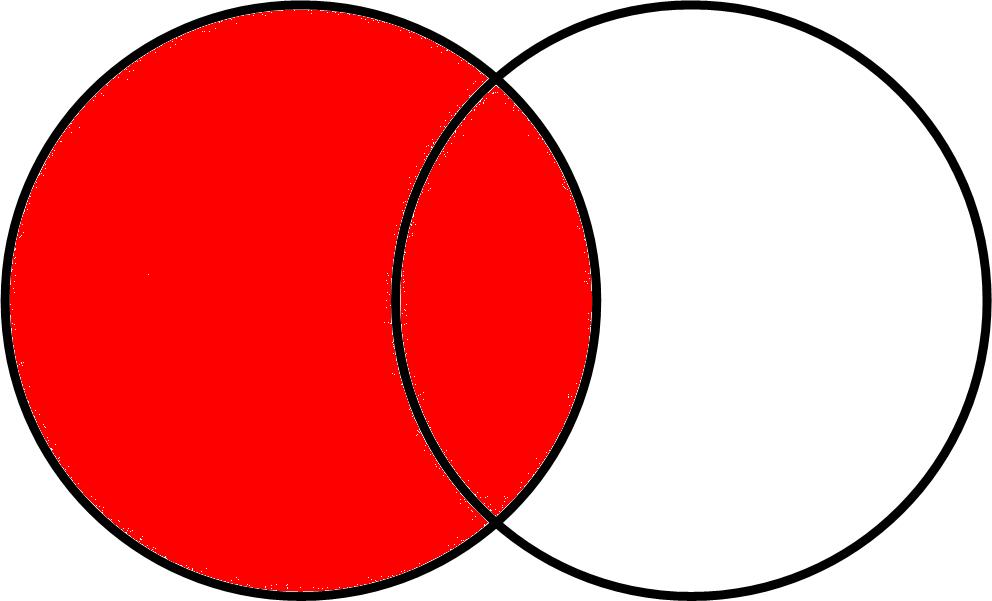
\includegraphics[height=2.862cm,width=4.725cm]{SetA.jpg}
  }
  \hspace{0.5cm} % Abstand zwischen den subfigures
  \subfigure[Set B]{
    \label{SET_B}
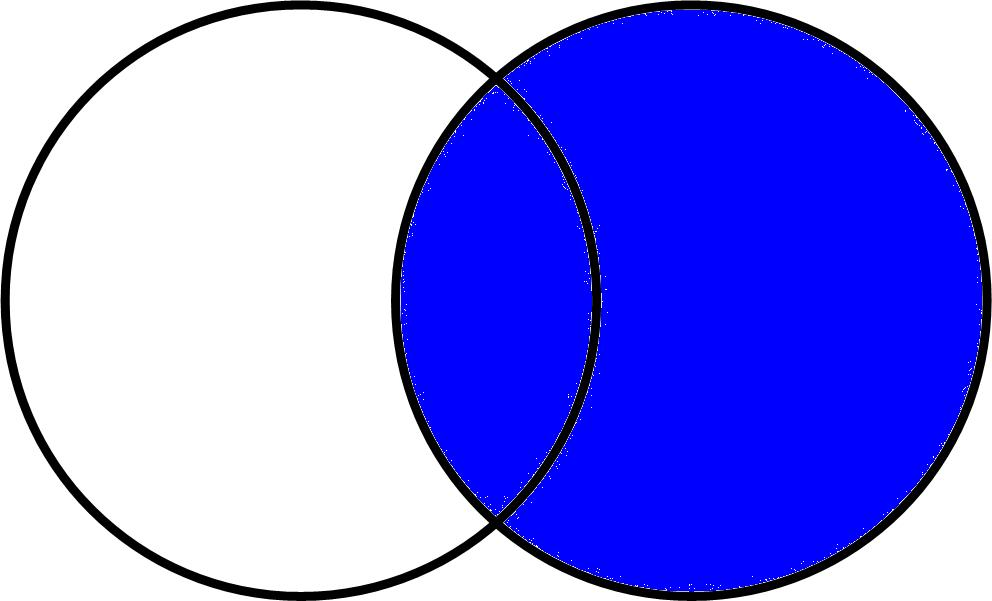
\includegraphics[height=2.862cm,width=4.725cm]{SetB.jpg}
	}  
  \hspace{0.5cm} % Abstand zwischen den subfigures
  \subfigure[Set A or set B $\;(A \cup B)$]{
    \label{SET_A_OR_SET_B}
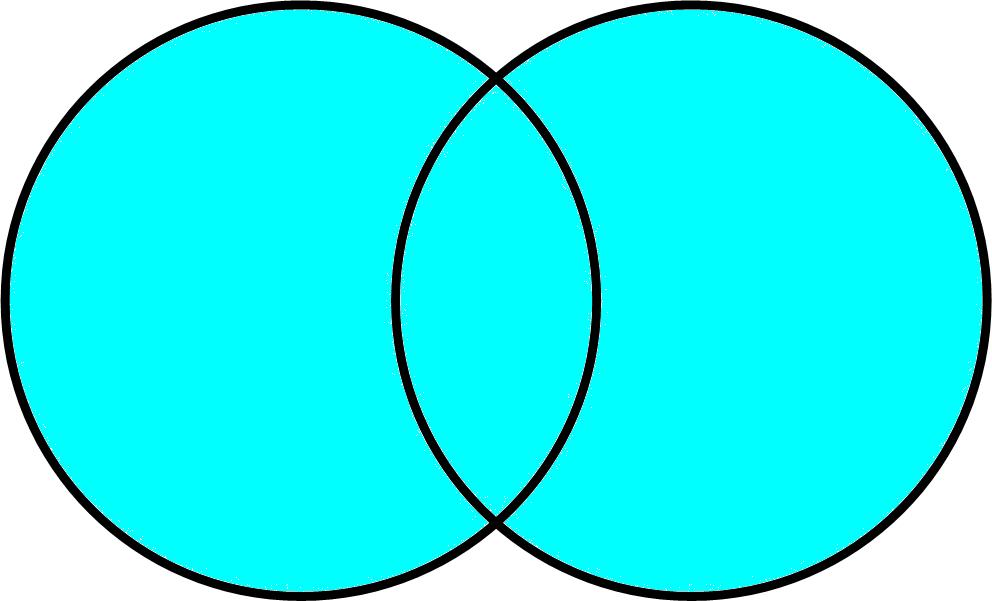
\includegraphics[height=2.862cm,width=4.725cm]{SetAOrB.jpg}
	}  

  \vspace{0.3cm} % Abstand zwischen den subfigures
  \subfigure[Set A and set B $\;(A \cap B)$]{
    \label{SET_A_AND_SET_B}
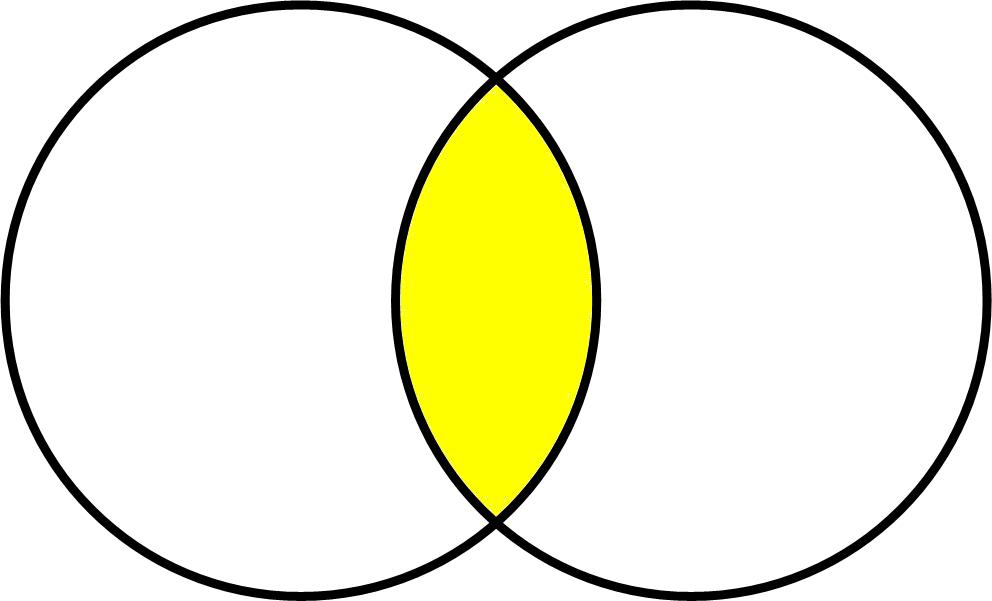
\includegraphics[height=2.862cm,width=4.725cm]{SetAAndB.jpg}
  }
  \hspace{0.5cm} % Abstand zwischen den subfigures
  \subfigure[Set A without set B $\;(A \setminus B)$]{
    \label{SET_A_WITHOUT_SET_B}
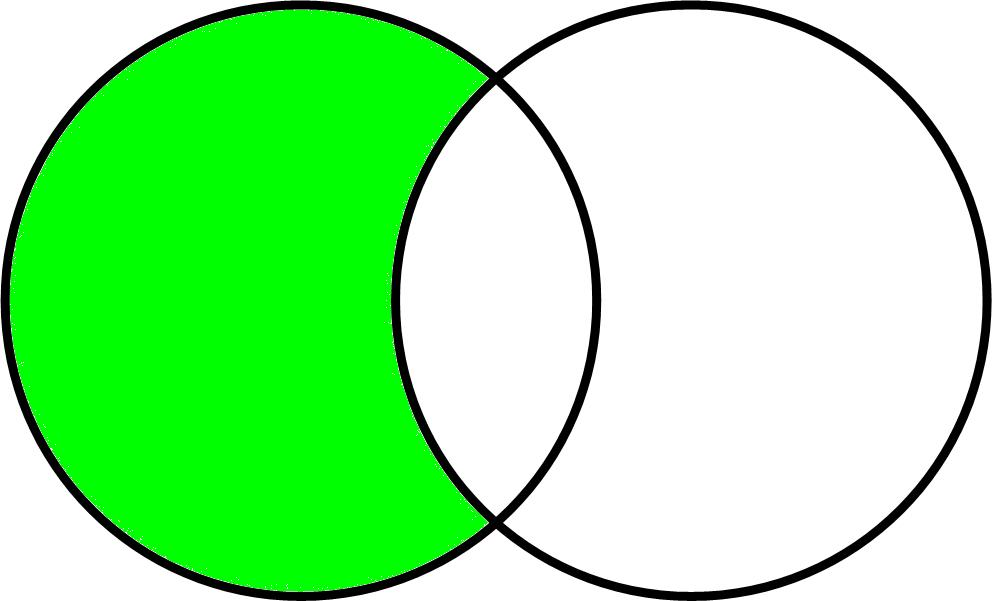
\includegraphics[height=2.862cm,width=4.725cm]{SetAOhneB.jpg}
	}  
  \hspace{0.5cm} % Abstand zwischen den subfigures
  \subfigure[Set B without set A $\;(B \setminus A)$]{
    \label{SET_B_WITHOUT_SET_A}
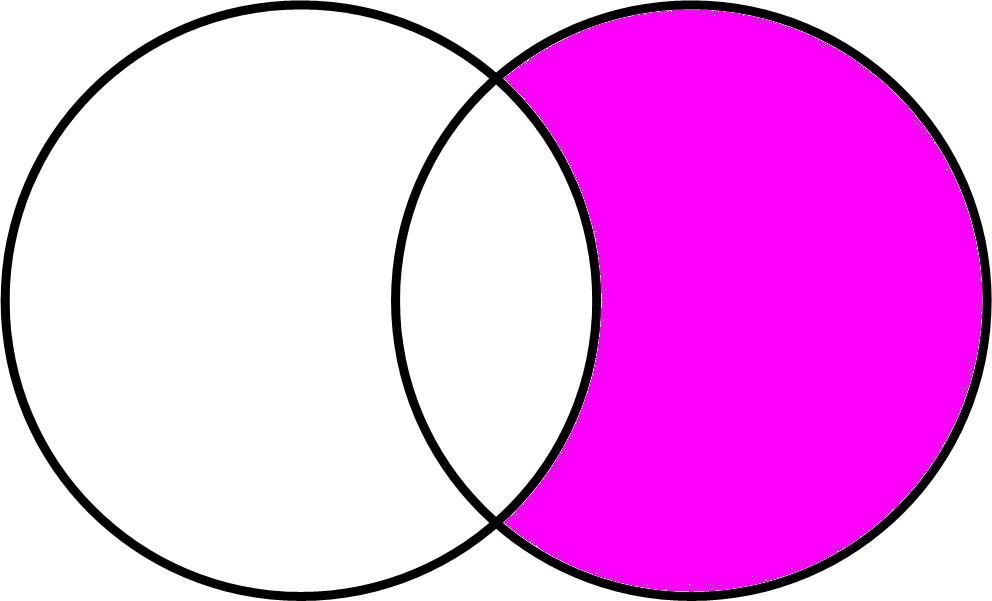
\includegraphics[height=2.862cm,width=4.725cm]{SetBOhneA.jpg}
	}  
 \vspace{0.3cm}
  \caption[Sets and their Boolean combinations]{Sets and their Boolean combinations}
  \label{BOOLEAN_COMBINATIONS_OF_SETS}
\end{figure}

If you created two primitives {\tt pythonOCC} can perform Boolean operations analog to those sketched in figure~\ref{BOOLEAN_COMBINATIONS_OF_SETS}.
Sometimes this is called {\it Constructive Solid Geometry (CSG)}.
You need to import {\tt OCC.BRepAlgoAPI} into your code because this functionality resides in that module.
The main functions are:
\begin{enumerate}
\item {\tt BRepAlgoAPI\_Fuse} combines two primitives so that the 
		resulting object occupies the space of both source objects. 
		This is equivalent to the {\tt or}-operation (symbol $\cup$) shown in
		figure~\ref{SET_A_OR_SET_B}.
\item {\tt BRepAlgoAPI\_Common} combines two primitives so that the 
		resulting object occupies the overlapping space of both source objects. 
		This is equivalent to the {\tt and}-operation (symbol $\cap$) shown in
		figure~\ref{SET_A_AND_SET_B}.
\item {\tt BRepAlgoAPI\_Cut} combines two primitives so that the 
		resulting object occupies the space of the first source object minus the 
		space ocuppied by the second source object. 
		This is equivalent to the {\tt without}-operation (symbol $\setminus$)
		shown in figures~\ref{SET_A_WITHOUT_SET_B} and~\ref{SET_B_WITHOUT_SET_A}.
\end{enumerate}

\subsection{A first sample on Boolean operations in pythonOCC}
In order to see how things work execute sample {\tt Step3\_1.py}, click on menu {\tt Draw} menu-item  {\tt draw sphere 1} and after that click on menu {\tt Draw} menu-item  {\tt draw sphere 2}.
Please note that before drawing the new object the screen is erased.
Use the new menu  {\tt Boolean} and select the menu-items.
Turn the objects so you can see their shape.

The menu-items should be self explaining so let's look at the code.
Listing~\ref{LISTING_STEP3_1_PY_A} shows how the menu and menu-items were changed to make the new funcionality available in the graphical use interface.
\begin{python}[moreemph={[4], 46, 48},caption={Step3\_1.py - Extending the menu},label=LISTING_STEP3_1_PY_A]
...
    # This is the place where we hook our functionality to menus
    # ----------------------------------------------------------
    add_menu('File')
    add_function_to_menu('File',  exit)
    add_menu('Draw')
    add_function_to_menu('Draw', draw_sphere_1)
    add_function_to_menu('Draw', draw_sphere_2)
    add_menu('Boolean')
    add_function_to_menu('Boolean', draw_fused_spheres)
    add_function_to_menu('Boolean', draw_cutted_spheres_1)
    add_function_to_menu('Boolean', draw_cutted_spheres_2)
    add_function_to_menu('Boolean', draw_common_spheres)
    add_menu('Erase')
    add_function_to_menu('Erase', erase_all)
...    
\end{python}
This should not be a suprise if you studied the code of the former steps.
So in the next step we do not discuss that anymore.
If you are unsure look at the code.

Listing~\ref{LISTING_STEP3_1_PY_B} shows two of the new functions added under menu {\tt Boolean}.
%
\begin{python}[moreemph={[4], 46, 48},caption={Step3\_1.py - Extending the functionality},label=LISTING_STEP3_1_PY_B]
def draw_cutted_spheres_2(event=None):
    # clear the display
    display.EraseAll()
    # create sphere
    Radius = 50.0
    # The sphere center as a Scipy array - 3 rows, one column
    # Note we use the scipy.zeros function
    PointZeroArray = scipy.zeros((3,1), dtype=float)
    MySphere1 = sphere_from_vector_and_radius(  PointZeroArray, 
                                                Radius )
    MySphere1Shape = MySphere1.Shape()

    # The sphere center as a Scipy array - 3 rows, one column
    MyPointAsArray = scipy.array([25.0, 50.0, 50.0])
    MyPointAsArray = scipy.reshape(MyPointAsArray,(3,1))
    MySphere2 = sphere_from_vector_and_radius(  MyPointAsArray, 
                                                Radius )
    MySphere2Shape = MySphere2.Shape()
    # Combine the spheres
    CuttedSpheres = OCC.BRepAlgoAPI.BRepAlgoAPI_Cut(    MySphere2Shape, 
                                                        MySphere1Shape )
    # Shape of combined spheres
    CuttedSpheres = CuttedSpheres.Shape()
    # Display 
    display.DisplayColoredShape( CuttedSpheres , 'BLUE' ) 

def draw_common_spheres(event=None):
    # clear the display
    display.EraseAll()
    # create sphere
    Radius = 50.0
    # The sphere center as a Scipy array - 3 rows, one column
    # Note we use the scipy.zeros function
    PointZeroArray = scipy.zeros((3,1), dtype=float)
    MySphere1 = sphere_from_vector_and_radius(  PointZeroArray, 
                                                Radius )
    MySphere1Shape = MySphere1.Shape()

    # The sphere center as a Scipy array - 3 rows, one column
    MyPointAsArray = scipy.array([25.0, 50.0, 50.0])
    MyPointAsArray = scipy.reshape(MyPointAsArray,(3,1))
    MySphere2 = sphere_from_vector_and_radius(  MyPointAsArray, 
                                                Radius )
    MySphere2Shape = MySphere2.Shape()
    # Combine the spheres
    CommonSpheres = OCC.BRepAlgoAPI.BRepAlgoAPI_Common( MySphere1Shape, 
                                                        MySphere2Shape )
    # Shape of combined spheres
    CommonSpheres = CommonSpheres.Shape()
    # Display 
    display.DisplayColoredShape( CommonSpheres , 'GREEN' ) 
...    
\end{python}
At the beginning of these functions the canvas is erased.
After that two sphere shapes are created in exactly the same manner as in listing \ref{LISTING_STEP2_2_PY_A}.
The next lines provide something new.
As the comment tells the spheres are combined.

Function {\tt draw\_cutted\_spheres\_2} performs the Boolean {\it without} operation utilising the function {\tt BRepAlgoAPI\_Cut}.
The function takes two shapes of primitives and delivers the result first primitive without second primitive.
If you change the order of the arguments given to function {\tt BRepAlgoAPI\_Cut} the Boolean operation is also changed like shown in function {\tt draw\_cutted\_spheres\_1}.

Next we look at function {\tt draw\_common\_spheres}.
Note that the function is similar to function {\tt draw\_cutted\_spheres\_2}.
The Boolean operation is the main difference between these functions.
In {\tt draw\_common\_spheres} function {\tt BRepAlgoAPI\_Common} is used to perform the {\tt and} operation.

Please note the similarity of both Boolean operations discussed.
Combing two primitives is always done in the same manner.
\begin{enumerate}
\item Construct {\tt Primitive\_1}
\item Create the shape {\tt Shape\_1 = Primitive\_1.Shape()}
\item Construct {\tt Primitive\_2}
\item Create the shape {\tt Shape\_2 = Primitive\_2.Shape()}
\item Perform the Boolean operation between {\tt Shape\_1} and  {\tt Shape\_2} to get a {\tt New\_Object}
\item Create {\tt New\_Object.Shape()} before displaying it
\end{enumerate}

\subsection{Extending the first sample on Boolean operations in pythonOCC}
\subsubsection{What we want to do and how it looks like}
Now that we know how to construct and combine primitives we should practice our new abilities.
What about drawing other things like a cylinder, a cone and an arrow?
Oh no, unfortunately there is no primitive creating arrows available.
So forget about the last one.
Stop!
We learned how to use Boolean operations so lets use a cone and a cylinder for the arrow and combine these.

Execute {\tt Step3\_2.py} to see how we extend our sample.
Please use menu {\tt Draw} and try the new functions {\tt draw cylinder},  {\tt draw cone} and  {\tt draw arrow}.
Also note that in contrast to {\tt Step3\_1.py} the functions under menu {\tt Draw} do not erase the canvas.
Hence all objects remain there until you use function {\tt erase all} or until you use one of the items under menu {\tt Boolean} or until you close the program.
Figure~\ref{STEP_3_2_SCREEN} shows how the canvas can look if you choose all objects from menu {\tt Draw}.
If you do the same you will see the objects but the perspective may differ.
% +++++++++++++++++++++++++++++++++++++++++++++++++++++++++++++++++++++++ 
% +++ Bild: Step 3_2 ++++++++++++++++++++++++++++++++++++++++++++++++++++
% +++++++++++++++++++++++++++++++++++++++++++++++++++++++++++++++++++++++ 
\begin{figure}[h]
\begin{center}
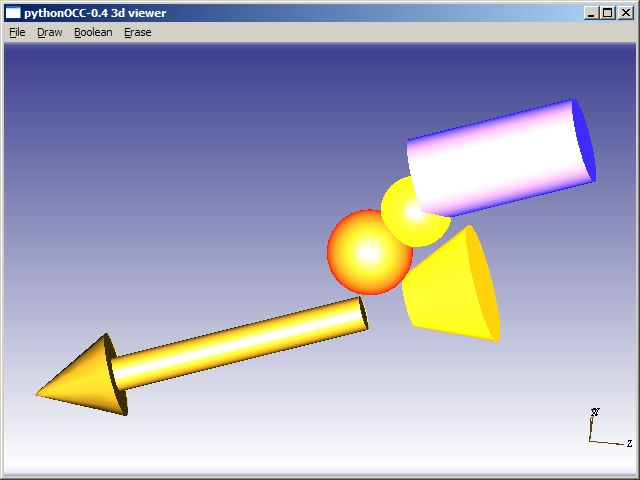
\includegraphics[height=8.5cm,width=11.3cm]{Step3_2.jpg}
\end{center}
\caption[Screenshot of Step3\_2]{\label{STEP_3_2_SCREEN}Screenshot of Step3\_2}
\end{figure}

\subsubsection{Creating a cylinder}
\label{SECT_CYLI}
We start with the creation of the cylinder object\footnote{
Maybe you ask yourself: Should I start learning how to use the OpenCascade documentation and practise beside working on that introduction?
If you want that open the  C++ documentation of Open~Cascade~\cite{OPENCASCADE_ORG} and read the constructors for a cylinder.
You don't need to do that now but you definitely have to do that if you create own applications.
So start using it whenever you think you are ready for it and learn how to go around in the docu. 
No fear! 
If you honor the structure shown in the C++ documentation and think in Python code you will learn using the application of the C++ documentation to create your own code although it is Python and not C++.
If you want to keep focused on what is presented here that's also ok. 
The intention of that hint is only to encourage the reader to use the documentation. 
To some extent the way of learning is different for every individual so you need to decide how to learn.}.
%
Listing~\ref{LISTING_STEP3_2_PY_A}\footnote{Please note the marvellous documentation strings. This is epytext a very easy markaup language for {\tt Epydoc}~\cite{EPYDOCWEB} a very efficient documentation tool. In my opinion it is worth a trial.}
presents the complete function.
Skim over it so we can go into the details in the following paragraphs.
%
\begin{python}[moreemph={[4], 46, 48},caption={Step3\_2.py - Defining a cylinder from a point, a direction vector, the length and the radius},label=LISTING_STEP3_2_PY_A]
def cylinder_from_point_directionvector_length_and_radius(  vector, 
                                                            directionvector,
                                                            length,
                                                            radius ):
    """
    Creates a cylinder utilising OCC.BRepPrimAPI.BRepPrimAPI_MakeCylinder out 
    of scipy arrays
    
    @param vector: vektor of starting point on the cylinder main axis
    @type  vector: scipy array(3,1)
    @param directionvector: direction vector of the cylinder main axis
    @type  directionvector: scipy array(3,1)
    @param length: cylinder length
    @type  length: float
    @param radius: cylinder radius
    @type  radius: float
    @return: cylinder

    sample::
    
        Vector = scipy.array([ 10.0, 10.0, 10.0 ])
        Vector = scipy.reshape( Vector, (3,1))
        
        TangUnitVector = scipy.array([  (1/scipy.sqrt(3)) , 
                                         1/scipy.sqrt(3)) , 
                                         1/scipy.sqrt(3)) ])
        TangUnitVector = scipy.reshape( TangUnitVector, (3,1))

        CylLength = 200
        CylRadius = 3
    
        Cyli = cylinder_from_point_directionvector_length_and_radius(Vector, 
                                                             TangUnitVector,
                                                             CylLength,
                                                             CylRadius ) 
        CyliShape = Cyli.Shape()
        display.DisplayColoredShape( CyliShape , 'RED' ) 
    """
    # Normalize the direction
    directionunitvector = NormVector(directionvector)
    # determine the second point
    vector2 = vector + length * directionunitvector    
    # components of vector in float values
    X1 = float( vector[ 0, 0] )
    Y1 = float( vector[ 1, 0] )
    Z1 = float( vector[ 2, 0] )
    # components of vector2 in float values
    X2 = float( vector2[ 0, 0] )
    Y2 = float( vector2[ 1, 0] )
    Z2 = float( vector2[ 2, 0] )
    # create OCC.gp.gp_Pnt-points
    P1 = OCC.gp.gp_Pnt( X1, Y1, Z1 )
    P2 = OCC.gp.gp_Pnt( X2, Y2, Z2 )
    # create direction unit vector from these points (not neccessary but if 
    # the directionunitvector is not of length 1 ...)
    directionP1P2 = scipy.array([   ( X2 - X1 ),
                                    ( Y2 - Y1 ),  
                                    ( Z2 - Z1 ) ])
    directionP1P2 = scipy.reshape( directionP1P2,(3,1))
    # distance between the points (X1, Y1, Z1) and (X2, Y2, Z2)
    length = length_column_vector(directionP1P2)
    # normalize direction
    directionP1P2 = NormVector(directionP1P2)                                                
    # origin at point 1 with OCC.gp.gp_Pnt
    origin_local_coordinate_system = OCC.gp.gp_Pnt( X1, Y1, Z1)
    # z-direction of the local coordinate system with OCC.gp.gp_Dir
    z_direction_local_coordinate_system = OCC.gp.gp_Dir(directionP1P2[0, 0], 
                                                        directionP1P2[1, 0], 
                                                        directionP1P2[2, 0])
    # local coordinate system with OCC.gp.gp_Ax2
    local_coordinate_system = OCC.gp.gp_Ax2(origin_local_coordinate_system, 
                                            z_direction_local_coordinate_system)
    # create cylinder utilising OCC.BRepPrimAPI.BRepPrimAPI_MakeCylinder
    cylinder = OCC.BRepPrimAPI.BRepPrimAPI_MakeCylinder(local_coordinate_system, 
                                                        radius, 
                                                        length, 
                                                        2 * scipy.pi )
    # return cylinder
    return cylinder
\end{python}
Function {\tt cylinder\_from\_point\_directionvector\_length\_and\_radius} is heavily commented so studying the code should be possible.
Anyhow a few words may help.
As the function name implies we construct the cylinder from a point, a direction vector, the length and the radius.
The first two parameters have to be {\tt Scipy} arrays the other two are floating point values.

We start with the normalization of the direction vector.
\begin{python}
    # Normalize the direction
    directionunitvector = NormVector(directionvector)
\end{python}
We utilize function {\tt NormVector} which uses function {\tt length\_column\_vector}.
Both functions are found in the source.
The first takes a direction vector of arbitrary length and returns a direction vector of length one with the same direction, the latter one determines the length of a vector.
\\
We get one center point at one end of the cylinder from the parameters.
So we compute the center point at the other end.
\begin{python}
    # determine the second point
    vector2 = vector + length * directionunitvector    
\end{python}
As already mentioned casting the contents of a {\tt Scipy} array to floats avoided some mysterious error messages.
Note that we do not mention that in the next sections. 
Please have a look at the following lines and try to keep them in mind.
\begin{python}
    # components of vector in float values
    X1 = float( vector[ 0, 0] )
    Y1 = float( vector[ 1, 0] )
    Z1 = float( vector[ 2, 0] )
\end{python}
The construction of points {\tt OCC.gp.gp\_Pnt} was already shown
\begin{python}
    # create OCC.gp.gp_Pnt-points
    P1 = OCC.gp.gp_Pnt( X1, Y1, Z1 )
\end{python}
but here is something new.
\begin{python}
    # z-direction of the local coordinate system with OCC.gp.gp_Dir
    z_direction_local_coordinate_system = OCC.gp.gp_Dir(directionP1P2[0, 0], 
                                                        directionP1P2[1, 0], 
                                                        directionP1P2[2, 0])
\end{python}
Thats the direction of the cylinder in {\tt pythonOCC} termonology.
It serves as a local $z$-coordinate for our cylinder primitive.
The constructor used a few lines later constructs a cylinder accoding to a local coordinate system.
The main axis of the cylinder created is the $z$-coordinate of that local coordinate system.
So it is no suprise that with
\begin{python}
    # local coordinate system with OCC.gp.gp_Ax2
    local_coordinate_system = OCC.gp.gp_Ax2(origin_local_coordinate_system, 
                                            z_direction_local_coordinate_system)
\end{python}
a local coordinate is introduced.
What about the $x$- and $y$-direction of the local coordinate system?
The answer is: I don't know.
But remember the cylinder is oriented along the $z$-axis and we do not care about $x$ and $y$.
The cross section of the cylinder is a circle so who cares about that?
\\
Now we are ready to create and return the cylinder object.
\begin{python}
    # create cylinder utilising OCC.BRepPrimAPI.BRepPrimAPI_MakeCylinder
    cylinder = OCC.BRepPrimAPI.BRepPrimAPI_MakeCylinder(local_coordinate_system, 
                                                        radius, 
                                                        length, 
                                                        2 * scipy.pi )
    # return cylinder
    return cylinder
\end{python}

We are in possession of a function creating cylinder objects.
Please read listing~\ref{LISTING_STEP3_2_PY_B} to see how we call it from function {\tt draw\_cylinder}.
\begin{python}[moreemph={[4], 46, 48},caption={Step3\_2.py - Calling the function defining a cylinder from a point, a direction vector, the length and the radius},label=LISTING_STEP3_2_PY_B]
def draw_cylinder(event=None):
    # cylinder radius
    Radius = 50.0
    # cylinder length
    Length = 200.0
    # The center point at one of the flat cylinder faces 
    Point = scipy.array([45.0, 80.0, 50.0])
    Point = scipy.reshape(Point,(3,1))
    # The direction of the cylinder from the point given above 
    DirectionFromPoint = scipy.array([25.0, 50.0, 150.0])
    DirectionFromPoint = scipy.reshape(DirectionFromPoint,(3,1))
    # create the cylinder object
    MyCylinder = cylinder_from_point_directionvector_length_and_radius( \
                                                       Point, 
                                                       DirectionFromPoint,
                                                       Length,
                                                       Radius )
    MyCylinderShape = MyCylinder.Shape()
    display.DisplayColoredShape( MyCylinderShape , 'BLUE' ) 
\end{python}
Do you recognize the similarity of that function to the functions used to call the function creating spheres?
It works exactly like those.

\subsubsection{Creating a cone}
\label{SECT_CONE}
If you followed the explainations of section~\ref{SECT_CYLI} you will easily get the cone too.
Have a look at code listing~\ref{LISTING_STEP3_2_PY_C}.
It shows the whole function.
Please read it and think about the similarity betwen listing \ref{LISTING_STEP3_2_PY_B} and~\ref{LISTING_STEP3_2_PY_C}.
Note that a cone is a cylinder exhibiting two different radi at the end so we need two radi to construct it.
\begin{python}[moreemph={[4], 46, 48},caption={Step3\_2.py - Function defining a cone from a point, a direction vector, the height and two radi},label=LISTING_STEP3_2_PY_C]
def cone_from_point_height_directionvector_and_two_radii( vector, 
                                                          directionvector,
                                                          height,
                                                          radius1,
                                                          radius2 ):
    """
    Creates a cone OCC.BRepPrimAPI.BRepPrimAPI_MakeCone.
        
    @param vector: vector at the beginning
    @type  vector: scipy array(3,1)
    @param directionvector: direction vector of the cone maina axis 
    @type  directionvector: scipy array(3,1)
    @param height: cone height
    @type  height: float
    @param radius1: radius at the cone bottom
    @type  radius1: float
    @param radius1: cone tip radius
    @type  radius1: float
    @return: cone 
    """
    # Normalize the direction
    directionunitvector = NormVector(directionvector)
    # Determine the second point
    vector2 = vector + height * directionunitvector    
    # components in floats
    X1 = float( vector[ 0, 0] )
    Y1 = float( vector[ 1, 0] )
    Z1 = float( vector[ 2, 0] )
    # components in floats
    X2 = float( directionunitvector[ 0, 0] )
    Y2 = float( directionunitvector[ 1, 0] )
    Z2 = float( directionunitvector[ 2, 0] )
    # create OCC.gp.gp_Pnt-point
    P1 = OCC.gp.gp_Pnt( X1, Y1, Z1 )
    # Read the direction unit vector (has to be done, but I do not know why)
    directionunit = scipy.array([   ( X2 ),
                                    ( Y2 ),  
                                    ( Z2 ) ])
    directionunit = scipy.reshape( directionunit,(3,1))
    # normalize - to be sure 
    directionunit = NormVector(directionunit)
    # origin at point 1 with OCC.gp.gp_Pnt
    origin_local_coordinate_system = OCC.gp.gp_Pnt( X1, Y1, Z1)
    # z-direction of the local coordinate system with OCC.gp.gp_Dir
    z_direction_local_coordinate_system = OCC.gp.gp_Dir(directionunit[0, 0], 
                                                        directionunit[1, 0], 
                                                        directionunit[2, 0])
    # local coordinate system with OCC.gp.gp_Ax2
    local_coordinate_system = OCC.gp.gp_Ax2(origin_local_coordinate_system, 
                                            z_direction_local_coordinate_system)

    # create cone utilising OCC.BRepPrimAPI.BRepPrimAPI_MakeCone
    cone = OCC.BRepPrimAPI.BRepPrimAPI_MakeCone(    local_coordinate_system, 
                                                    radius1, 
                                                    radius2, 
                                                    height )
    # return cone
    return cone
\end{python}
I think the comments given in the code above are sufficient.
Also the call of the function should be clear if you have a look at the source. So lets go ahead to combine the cone and the cylinder.

\subsubsection{Creating an arrow}
\label{SECT_ARROW}
Creation of an arrow ist straightforward with what we've learned until now.
As in section~\ref{SECT_CYLI} the arrow creating function is given first and after that the interesting lines are discussed.
Look at listing~\ref{LISTING_STEP3_2_PY_D}. 
\begin{python}[moreemph={[4], 46, 48},caption={Step3\_2.py - Function defining an arrow shape object from a point, a direction vector, the arrow length, the radius of the arrow shaft, the length of the arrow head and the radius of the arrow head},label=LISTING_STEP3_2_PY_D]
def arrowShape( vector, 
                directionvector,
                arrowlength,
                radius_of_arrow_shaft,
                lenght_of_arrow_head,
                radius_of_arrow_head ):
    '''
    Function arrowshape creates the shape of an arrow starting at vector
    pointing into diretcion. We create a cylinder and a cone and combine the 
    utilising OCC.BRepAlgoAPI.BRepAlgoAPI_Fuse.

    @param vector: starting point of the arrow
    @type  vector: scipy array(3,1)
    @param directionvector: direction of the arrow
    @type  directionvector: scipy  array(3,1)
    @param arrowlength: length of the arrow
    @type  arrowlength: scalar
    @param radius_of_arrow_shaft: radius of the arrow shaft
    @type  radius_of_arrow_shaft: scalar
    @param lenght_of_arrow_head: length of the arrow head
    @type  lenght_of_arrow_head: scalar
    @param radius_of_arrow_head: radius of the arrow head
    @type  radius_of_arrow_head: scalar
    @return: Pfeil als Shape Objekt
    '''
    # Normalize the direction
    directionunitvector = NormVector(directionvector)
    # the shaft length
    cylinder_length = arrowlength - lenght_of_arrow_head
    # create shaft
    arrow_shaft = cylinder_from_point_directionvector_length_and_radius( \
                                                    vector, 
                                                    directionunitvector,
                                                    cylinder_length,
                                                    radius_of_arrow_shaft ) 
    arrow_shaft_Shape = arrow_shaft.Shape()
    # begin of arrow head (flat suface)
    arrow_head_point = vector + cylinder_length * directionunitvector
    # create arrow head
    arrow_head = cone_from_point_height_directionvector_and_two_radii(  \
                                                    arrow_head_point, 
                                                    directionunitvector,
                                                    lenght_of_arrow_head,
                                                    radius_of_arrow_head,
                                                    0.0 )
    arrow_head_Shape = arrow_head.Shape()
    # combine shaft and head
    arrow = OCC.BRepAlgoAPI.BRepAlgoAPI_Fuse(   arrow_shaft_Shape, 
                                                arrow_head_Shape )       
    arrowShape = arrow.Shape() 
    # return Shape of the arrow
    return arrowShape
\end{python}
Did you recognize the different return type here?
In code listing \ref{LISTING_STEP3_2_PY_B} and \ref{LISTING_STEP3_2_PY_C} we returned the geometric object here we return the shape of the object.
Why do we do that?
Only to demonstrate that it is also possible to return the shape of the object.

We start our examination with a look at figure~\ref{STEP_3_2_SCREEN}.
Our arrow consists of a cylindrical shaft and a conic head.
The heads cone has two radi.
One of it is zero.
That's the tip of the arrow.
The other one is larger than the radius of the cylindrical shaft.

The first lines of  code listing \ref{LISTING_STEP3_2_PY_D} build the cylinder shape of the shaft.
To get the length of the shaft we subtract the length of the head from the total length of the arrow.
Both values are given in the parameter set.
\begin{python}
    # Normalize the direction
    directionunitvector = NormVector(directionvector)
    # the shaft length
    cylinder_length = arrowlength - lenght_of_arrow_head
    # create shaft
    arrow_shaft = cylinder_from_point_directionvector_length_and_radius( \
                                                    vector, 
                                                    directionunitvector,
                                                    cylinder_length,
                                                    radius_of_arrow_shaft ) 
    arrow_shaft_Shape = arrow_shaft.Shape()
\end{python}
Next the shape of the conic head is constructed.
We need to compute the beginning of the cone so we walk the length of the shaft from the starting point of the arrow into the arrows direction to reach the flat side of the conic arrow head.
Here we create the cone which has one radius of zero.
I simply tried which radius is the right one.
That's the way things can be solved if you are to lazy for studying the documentation.
\begin{python}
    # begin of arrow head (flat suface)
    arrow_head_point = vector + cylinder_length * directionunitvector
    # create arrow head
    arrow_head = cone_from_point_height_directionvector_and_two_radii(  \
                                                    arrow_head_point, 
                                                    directionunitvector,
                                                    lenght_of_arrow_head,
                                                    radius_of_arrow_head,
                                                    0.0 )
    arrow_head_Shape = arrow_head.Shape()
\end{python}
Both shapes, the cylinder shape and the cone shape, are then glued together to form the arrow object.
See how easy it is to construct new objects with the aid of Boolean operations. 
\begin{python}
    # combine shaft and head
    arrow = OCC.BRepAlgoAPI.BRepAlgoAPI_Fuse(   arrow_shaft_Shape, 
                                                arrow_head_Shape )       
\end{python}
As already mentioned in that function we do not return the object we return its shape.
Whether there are advatages or disadvantages between returning the shape or the object I cannot tell.
But as you can see both options deliver the same result.
\begin{python}
    arrowShape = arrow.Shape() 
    # return Shape of the arrow
    return arrowShape
\end{python}
Note if you return the shape to a calling function this calling function must not call the {\tt Shape()} method again.
If it does that a error will happen.


If you cannot imagine how the function is called and how the shape is drawn please look at the code.
Function {\tt draw\_arrow} which is hooked into the menu does the job in exactly the same manner as the one building the spheres, the cylinder and the cone.
These functions define the needed parameters, call the appropriate function to create the object and display the shape of the created object. 

This was much more a jump then a step. 
If you got that  so far you are at least prepared for discussions dealing with {\it Constructive solid geometry (CSG)} and  {\it Boolean operations}.
That's not so bad!

\section{Step 4 - Time for Practice}
\subsection{Extending our sample}
The last sample of the former section is now used as a starting point for getting some practice.

Did you notice the little coordinate cross at the bottom of the screen? 
It shows you the $x$-, $y$- and $z$-direction in the displayed space.
To get some practice we place a larger coordinate cross at the origin.
Execute {\tt Step4\_1.py}, click on menu {\tt Draw} menu-item  {\tt draw coordinates} to get the screen shown in figure~\ref{STEP_4_1_SCREEN}.
% +++++++++++++++++++++++++++++++++++++++++++++++++++++++++++++++++++++++ 
% +++ Bild: Step 4_1 ++++++++++++++++++++++++++++++++++++++++++++++++++++
% +++++++++++++++++++++++++++++++++++++++++++++++++++++++++++++++++++++++ 
\begin{figure}[h]
\begin{center}
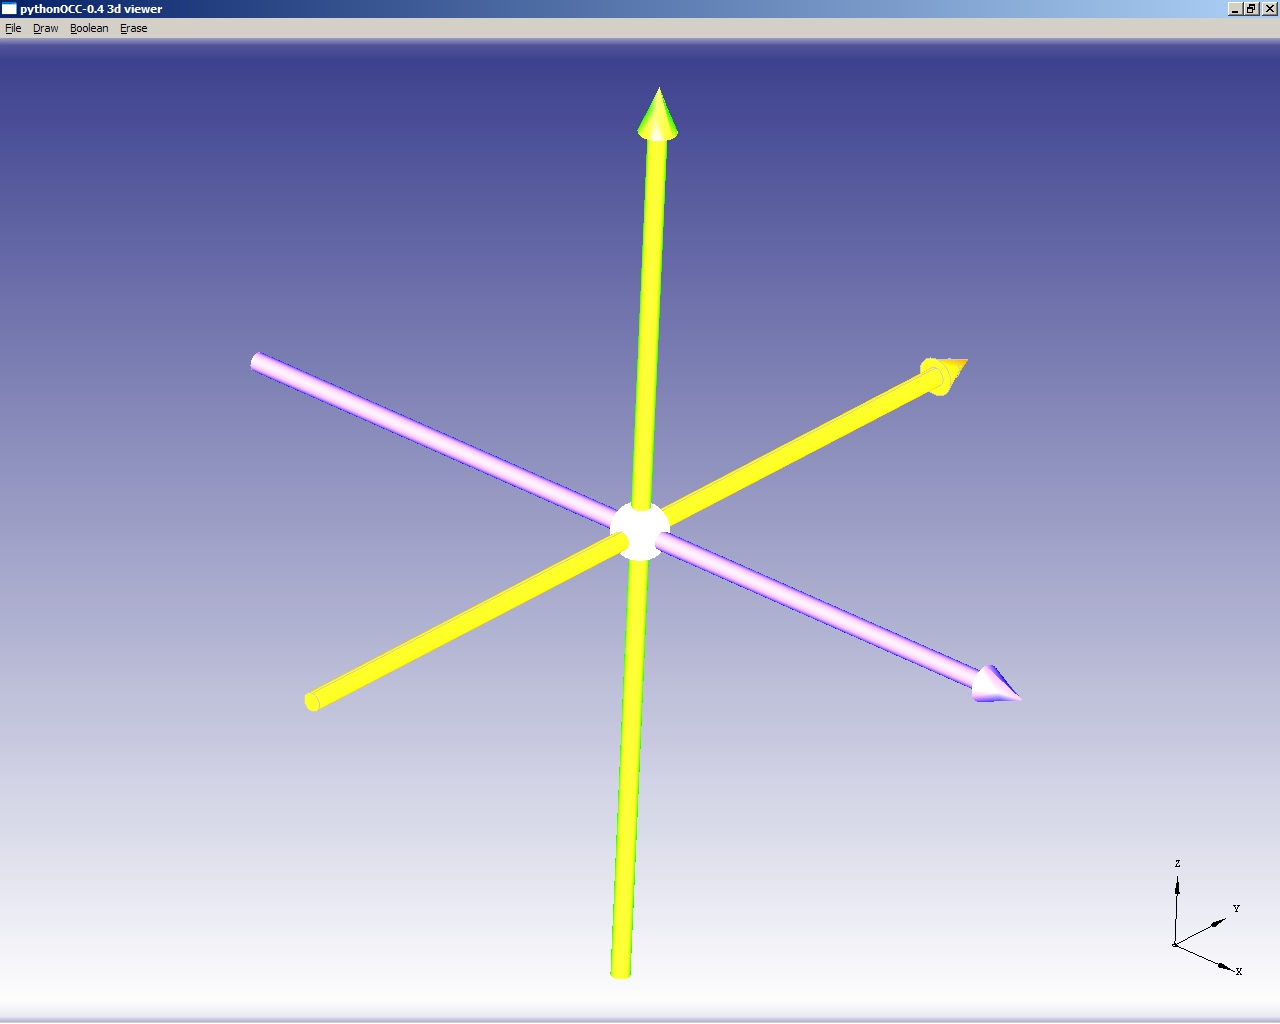
\includegraphics[height=8.5cm,width=11.3cm]{Step4_1.jpg}
\end{center}
\caption[Screenshot of Step4\_1]{\label{STEP_4_1_SCREEN}Screenshot of Step4\_1}
\end{figure}

To see how this is done start reading Listing~\ref{LISTING_STEP4_1_PY_A} where the function which is called after selecting that menu item is presented.
The function is heavily commented and should be understood without difficulty.
%
\begin{python}[moreemph={[4], 46, 48},caption={Step4\_1.py - Drawing a larger, coloured coordinate system -- function {\tt draw\_coordinates} which is called by clicking on the menu},label=LISTING_STEP4_1_PY_A]
def draw_coordinates(event=None):
    # The radius of a sphere at the origin
    centerpoint_sphere_radius = 30.0
    # The length of every axis starting at -length/2 and ending at length/2
    arrowlength = 1000.0
    # Radius of the arrow shaft of every axis
    radius_of_arrow_shaft = 10.0
    # Length of every axis
    lenght_of_arrow_head = 50.0
    # Radius of the arrow heads cone
    radius_of_arrow_head = 20.0
    # Create the Coordinate and Draw it
    CoordinateCrossShape(   centerpoint_sphere_radius,
                            arrowlength,
                            radius_of_arrow_shaft,
                            lenght_of_arrow_head,
                            radius_of_arrow_head )
\end{python}

Function {\tt draw\_coordinates} calls {\tt CoordinateCrossShape}.
We should also have a look at that function given in Listing~\ref{LISTING_STEP4_1_PY_B}.
Before you start reading the code let me state that all the functionality used in that function was already explained in the last section.
I also like to mention that the different parts of the coordinate cross are not combined by Boolean functions.
On one hand this makes it easy to apply different colours to the single parts on the other there is no need to move or turn the coordinate axis - these are our world coordinates.
Finally I would like to guide your attention at the end of the function.
It does not return anything.
The function itself draws the coordinate cross.
%
\begin{python}[moreemph={[4], 46, 48},caption={Step4\_1.py - Drawing a coordinate system -- function {\tt CoordinateCrossShape} which is called by function {\tt draw\_coordinates}},label=LISTING_STEP4_1_PY_B]
def CoordinateCrossShape(   centerpoint_sphere_radius,
                            arrowlength,
                            radius_of_arrow_shaft,
                            lenght_of_arrow_head,
                            radius_of_arrow_head ):
    '''
    Function arrowshape creates the shape of an arrow starting at vector
    pointing into diretcion. We create a cylinder and a cone and combine the 
    utilising OCC.BRepAlgoAPI.BRepAlgoAPI_Fuse.

    @param vector: starting point of the arrow
    @type  vector: scipy array(3,1)
    @param directionvector: direction of the arrow
    @type  directionvector: scipy  array(3,1)
    @param arrowlength: length of the arrow
    @type  arrowlength: scalar
    @param radius_of_arrow_shaft: radius of the arrow shaft
    @type  radius_of_arrow_shaft: scalar
    @param lenght_of_arrow_head: length of the arrow head
    @type  lenght_of_arrow_head: scalar
    @param radius_of_arrow_head: radius of the arrow head
    @type  radius_of_arrow_head: scalar
    @return: Arrow as Shape object
    '''
    # The origin of the coordinate system
    Origin = scipy.zeros((3,1),dtype=float)
    # The direction unit vectors of the axis
    xDir = scipy.zeros((3,1),dtype=float)
    xDir[0,0] = 1.0
    yDir = scipy.zeros((3,1),dtype=float)
    yDir[1,0] = 1.0
    zDir = scipy.zeros((3,1),dtype=float)
    zDir[2,0] = 1.0
    
    # Create the center point sphere shape at the origin
    OriginSphere = sphere_from_vector_and_radius(   Origin, 
                                                    centerpoint_sphere_radius )
    OriginSphereShape = OriginSphere.Shape()

    # Create the XAxis shape
    XAxisShape = arrowShape(    Origin - 0.5 * arrowlength * xDir, 
                                xDir,
                                arrowlength,
                                radius_of_arrow_shaft,
                                lenght_of_arrow_head,
                                radius_of_arrow_head )
    # Create the YAxis shape
    YAxisShape = arrowShape(    Origin - 0.5 * arrowlength * yDir, 
                                yDir,
                                arrowlength,
                                radius_of_arrow_shaft,
                                lenght_of_arrow_head,
                                radius_of_arrow_head )
    # Create the ZAxis shape
    ZAxisShape = arrowShape(    Origin - 0.5 * arrowlength * zDir, 
                                zDir,
                                arrowlength,
                                radius_of_arrow_shaft,
                                lenght_of_arrow_head,
                                radius_of_arrow_head )
    
    # Display these shapes
    display.DisplayColoredShape( OriginSphereShape , 'WHITE' ) 
    display.DisplayColoredShape( XAxisShape , 'BLUE' ) 
    display.DisplayColoredShape( YAxisShape , 'ORANGE' ) 
    display.DisplayColoredShape( ZAxisShape , 'GREEN' ) 
\end{python}

Why is it possible to draw on the display without receiving it as a parameter?
The reason is that the display is created outside of a class or function.
Look at the end of {\tt Step4\_1.py} which is shown in  Listing~\ref{LISTING_STEP4_1_PY_C}.
%
\begin{python}[moreemph={[4], 46, 48},caption={Step4\_1.py - Creating the display},label=LISTING_STEP4_1_PY_C]
if __name__ == '__main__':
    # OCC.Display.SimpleGuiinit_display() returns multiple
    # values which are assigned here
    display, start_display, add_menu, add_function_to_menu = \
        OCC.Display.SimpleGui.init_display()
...
    start_display()
\end{python}

\subsection{Time for Housekeeping}
Our sample became pretty large.
So lets divide it into two parts:
\begin{description}
\item [{\tt Step4\_2.py}] the main program and
\item [{\tt Step4\_2\_A.py}] a module containing the Scipy stuff and the construction of geometric objects.
\end{description}
Run program {\tt Step4\_2.py} and see that it works exactly like {\tt Step4\_1.py}.
Sure you know how this division works.
We simply took some functions from {\tt Step4\_1.py} and put these into a module called {\tt Step4\_2\_A.py}.
The remaining main script is called {\tt Step4\_2.py}.
In order to tell Python where to look for the outsourced functions we add
\begin{python}
...    
from Step4_2_A import *
...    
\end{python}
at the beginning of {\tt Step4\_2.py}.
Now have a closer look at {\tt Step4\_2\_A.py}.
See that we also modified function {\tt CoordinateCrossShape}.
Look at the function definition we added one parameter. 
It is the parameter {\tt display}.
\begin{python}
def CoordinateCrossShape(   display, 
                            centerpoint_sphere_radius,
                            arrowlength,
                            radius_of_arrow_shaft,
                            lenght_of_arrow_head,
                            radius_of_arrow_head ):
...    
\end{python}
You should also notice that the function call which is done from {\tt Step4\_2.py} uses that additional parameter too.
Of course, we need a structure of parameters which reflects the parameter line of the function called.
\begin{python}
...    
    # Create the Coordinate and Draw it
    CoordinateCrossShape(   display, 
                            centerpoint_sphere_radius,
                            arrowlength,
                            radius_of_arrow_shaft,
                            lenght_of_arrow_head,
                            radius_of_arrow_head )
...    
\end{python}
Why do we have to do that?
Think about a painter painting for some client.
If the client and the painter are in the same room they can point on the canvas to be painted easily.
If these two, the painter and the client, are talking via a phone line and the painter is not in the clients room containing the canvas the client needs to specify his canvas so the painter knows on where to go and paint on.
Note that the painter probably has different clients all of them have their own canvas in their room and all of them may ask the painter to come around and paint on their canvas.
The same is true here. 

\subsection{Once more: Extending the sample}
In this section only a few thing to learn were introduced so far.
Hence we should have a brief look at something not mentioned until now.

We already saw that we can write code like 
\begin{python}
...    
    display.DisplayColoredShape( MyCylinderShape , 'YELLOW' ) 
...    
\end{python}
to draw coloured objects.
What if we like to change other things like material and transparency?
Here the coding gets a little more complicated because we need to be familiar with the {\it Application Interactive Services (AIS)}.
These services are responsible for the presentation including display properties of geometrical structures, display quality, detection and selection.

At the moment I cannot tell how all this can be done and I need to explore the  {\it Application Interactive Services (AIS)} to see how to make use of them.
Nevertheless I want to tell you my actual knowledge which may help you to get things done if you try to make objects transparent and so on. 

Execute {\tt Step4\_3.py} and choose menu {\tt Draw}, menu item {\tt draw cylinder}.
Probably you cannot see the cylinder without moving away from the scene with the mouse.
As an alternative choose menu {\tt Draw}, menu item {\tt draw coordinates} so all objects are shown.
The same is true if you select menu {\tt Draw}, menu item {\tt draw cone}.
I cannot tell how this can be avoided but I will add the solution in some future revision of this document if I'll find any.
Select also  menu {\tt Draw}, menu item {\tt draw sphere 2}.
See that the cylinder intersects with sphere~2.
The cylinder is transparent and sphere~2 can be seen through the cylinder.
In addition the material of the cone is modified compared to the display in {\tt Step4\_2.py}.
Figure~\ref{STEP_4_3_SCREEN} shows the screen presented after you reproduced the steps above.
% +++++++++++++++++++++++++++++++++++++++++++++++++++++++++++++++++++++++ 
% +++ Bild: Step 4_3 ++++++++++++++++++++++++++++++++++++++++++++++++++++
% +++++++++++++++++++++++++++++++++++++++++++++++++++++++++++++++++++++++ 
\begin{figure}[h]
\begin{center}
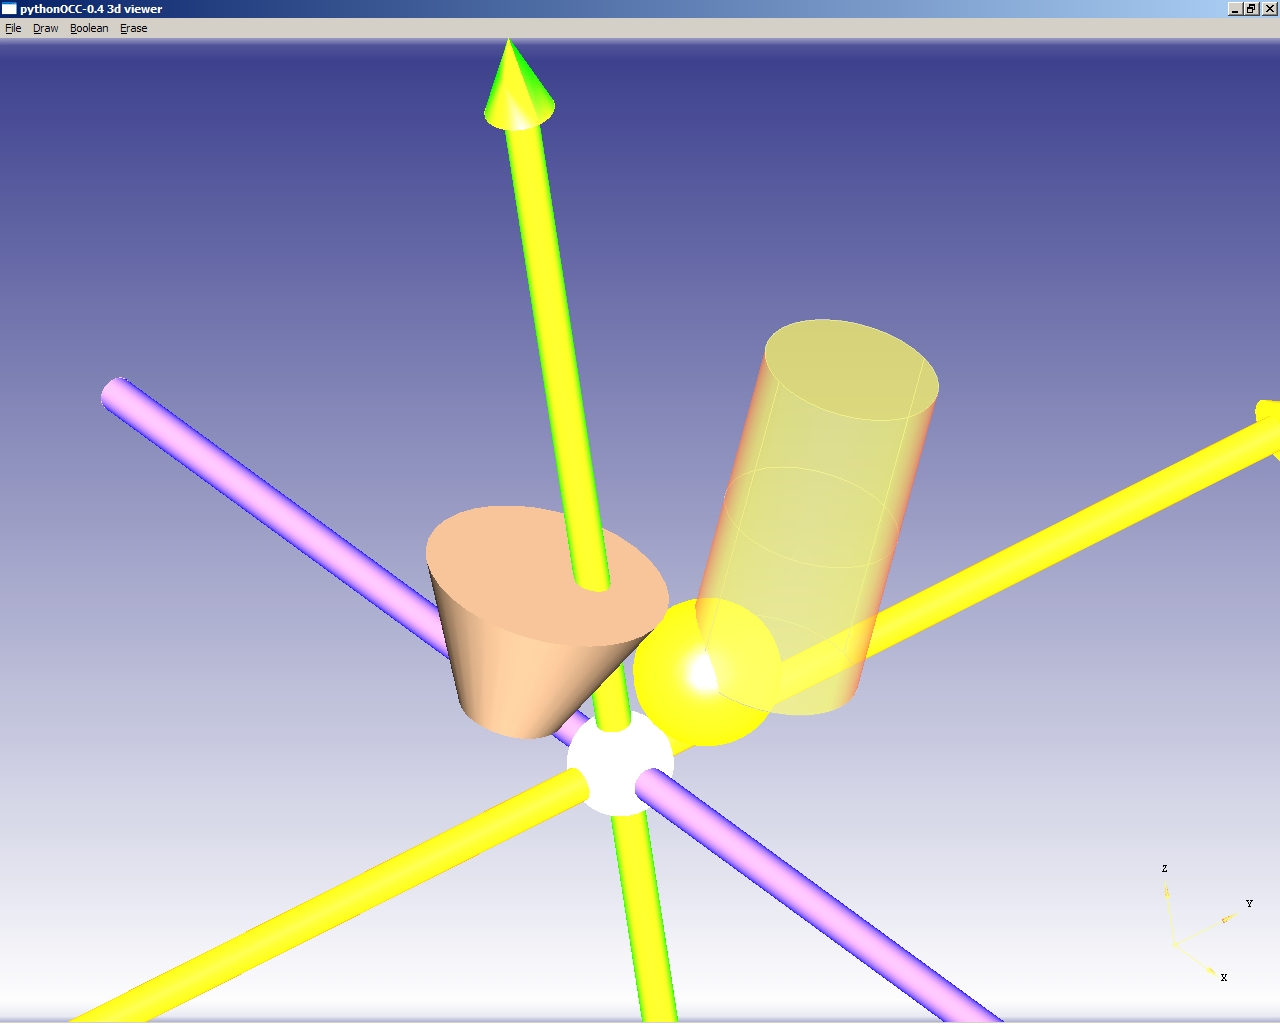
\includegraphics[height=8.5cm,width=11.3cm]{Step4_3.jpg}
\end{center}
\caption[Screenshot of Step4\_3]{\label{STEP_4_3_SCREEN}Screenshot of Step4\_3}
\end{figure}

Listing~\ref{LISTING_STEP4_3_PY} shows the modifications starting at the beginning of {\tt Step4\_3.py} and both, the modified cone and the modified cylinder display.
As already mentioned this sample is not fully understood by me so I only can show how I got it to work.
%
\begin{python}[moreemph={[4], 46, 48},caption={Step4\_1.py - Creating the display},label=LISTING_STEP4_3_PY]
...
from OCC.AIS import *
from OCC.Quantity import *
from OCC.Graphic3d import *
...
def draw_cylinder(event=None):
    # cylinder radius
    Radius = 50.0
    # cylinder length
    Length = 200.0
    # The center point at one of the flat cylinder faces 
    Point = scipy.array([45.0, 80.0, 50.0])
    Point = scipy.reshape(Point,(3,1))
    # The direction of the cylinder from the point given above 
    DirectionFromPoint = scipy.array([25.0, 50.0, 150.0])
    DirectionFromPoint = scipy.reshape(DirectionFromPoint,(3,1))
    # create the cylinder object
    MyCylinder = cylinder_from_point_directionvector_length_and_radius( \
                                                            Point, 
																				DirectionFromPoint,
                                                            Length,
                                                            Radius )
    MyCylinderShape = MyCylinder.Shape()
    
    ais_shape_MyCylinderShape = AIS_Shape( MyCylinderShape ).GetHandle()
    ais_context = display.GetContext().GetObject()
    ais_context.SetColor(  ais_shape_MyCylinderShape,  Quantity_NOC_TOMATO )
    ais_context.SetTransparency( ais_shape_MyCylinderShape, 0.3, True)
    ais_context.Display( ais_shape_MyCylinderShape ) 

def draw_cone(event=None):
    # cone radius 1
    Radius1 = 30.0
    # cone radius 2
    Radius2 = 70.0
    # cone height
    Height = 90.0
    # The center point at one of the flat cone faces 
    Point = scipy.array([-25.0, -50.0, 50.0])
    Point = scipy.reshape(Point,(3,1))
    # The direction of the cone from the point given above 
    DirectionFromPoint = scipy.array([25.0, 50.0, 150.0])
    DirectionFromPoint = scipy.reshape(DirectionFromPoint,(3,1))
    # create the cone object
    MyCone = cone_from_point_height_directionvector_and_two_radii( \
                                                            Point, 
                                                            DirectionFromPoint,
                                                            Height,
                                                            Radius1,
                                                            Radius2 )

    MyConeShape = MyCone.Shape()
    ais_shape_MyConeShape = AIS_Shape( MyConeShape ).GetHandle()
    ais_context = display.GetContext().GetObject()
    ais_context.SetMaterial(    ais_shape_MyConeShape,  
                                Graphic3d.Graphic3d_NOM_STONE )
    ais_context.Display( ais_shape_MyConeShape ) 
\end{python}

%\section{Step 5 - A 3D Function}
\subsection{See the result}
In this section we want to draw a function in 3D.
Our function is a spiral around the $z$-axis.
At some points the functions tangent vectors are displayed.
In order to give you an image what we want to create I present the result of our subject in figure~\ref{STEP_5_1_SCREEN}.
Subfigure~\ref{STEP_5_1_1_SCREEN} shows the spiral function and the coordinate cross invented in the last section.
In order to show the spatial property of the spiral subfigure~\ref{STEP_5_1_2_SCREEN} shows a cylinder with the same radius and orientation as the spiral.
% +++++++++++++++++++++++++++++++++++++++++++++++++++++++++++++++++++++++ 
% +++ Bild: Step 5_1 ++++++++++++++++++++++++++++++++++++++++++++++++++++
% +++++++++++++++++++++++++++++++++++++++++++++++++++++++++++++++++++++++ 
\begin{figure}[htbp]
  \centering
  \subfigure[Screenshot of Step5\_1 without the cylinder]{
    \label{STEP_5_1_1_SCREEN}
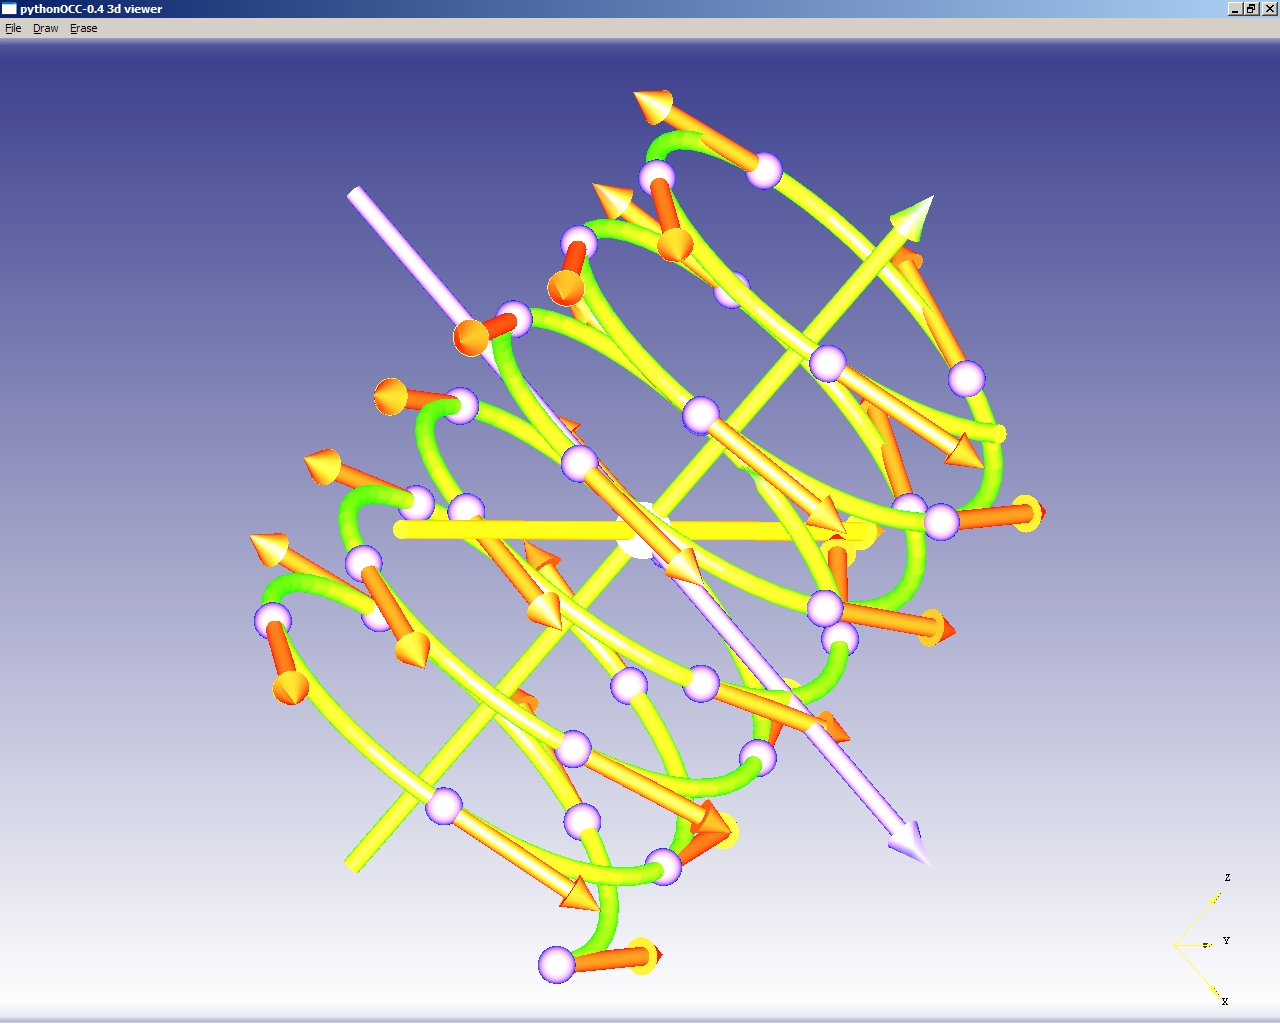
\includegraphics[height=8.5cm,width=11.3cm]{Step5_1_1.jpg}
  }

  \vspace{0.3cm} % Abstand zwischen den subfigures
  \subfigure[Screenshot of Step5\_1 with the cylinder]{
    \label{STEP_5_1_2_SCREEN}
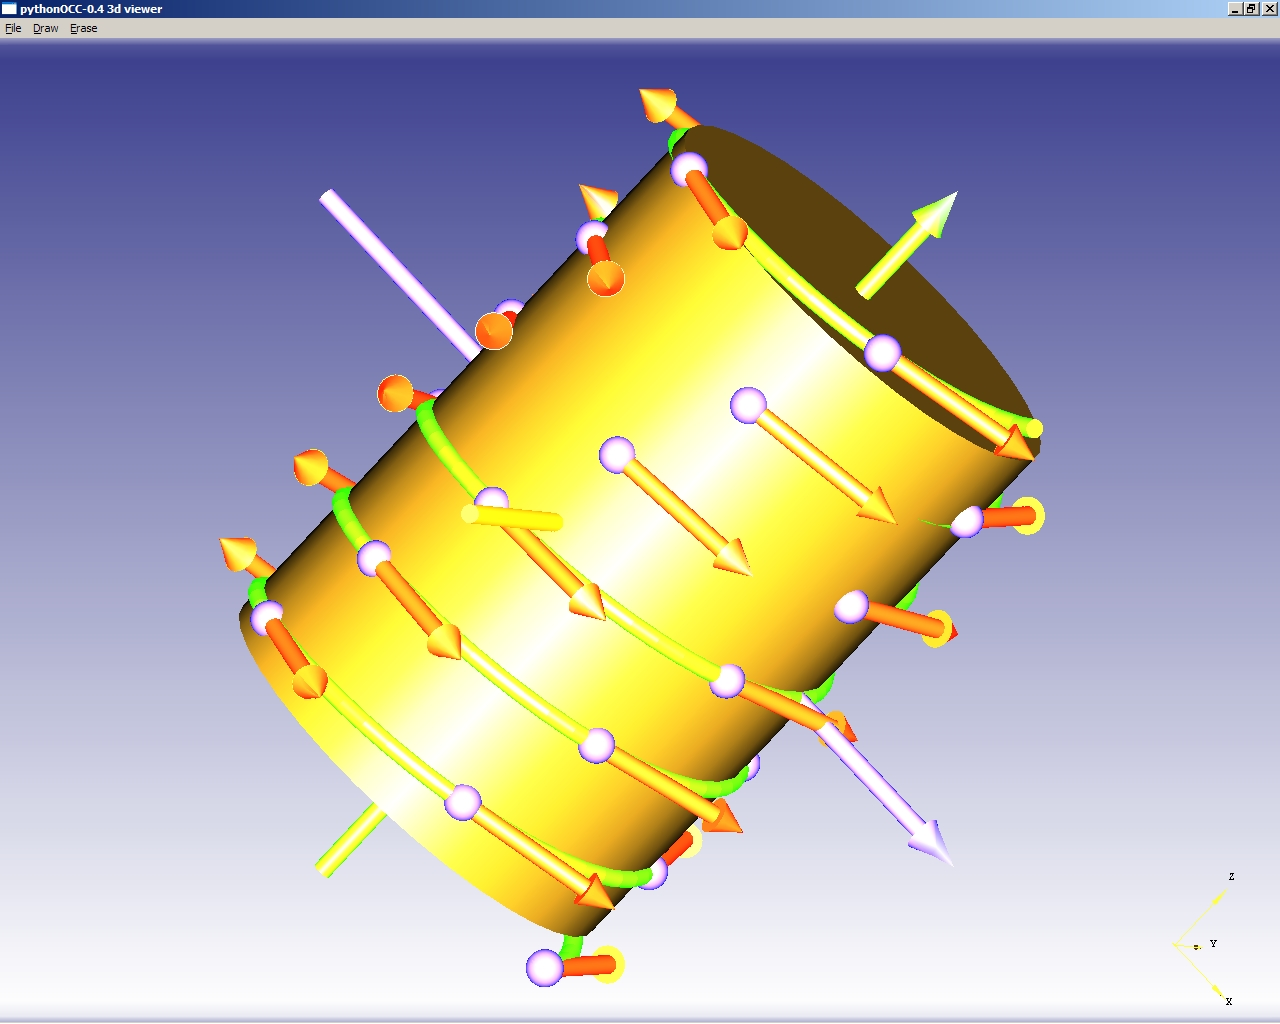
\includegraphics[height=8.5cm,width=11.3cm]{Step5_1_2.jpg}
  }

 \vspace{0.3cm}
  \caption[Screenshots of Step5\_1]{Screenshots of Step5\_1}
  \label{STEP_5_1_SCREEN}
\end{figure}

\subsection{Some formulars}
If you do not know how to construct a spiral and how to compute its tangent vector at a certain point, here is a short presentation of the formulars needed\footnote{It is not my aim to explain maths. Please search on the web or consult a book if you do not understand that. My aim is to give you an example how to draw a fuction in 3D. So if you do not care about math that does not hurt. If you want your functions to be shown take this sample as a template.}.

If you look at a spiral from the top you see a circle if you do not take the perspective into account.
Hence it is no suprise that if we want to create a spiral around the $z$-direction the $x$- and $y$-components of the function create a circle.
Due to the spiral should be regular the $z$-component is a linear function.
So we can write down the formular for our spiral to
\begin{equation}
\label{EQSPIRAL}
\mathbf{C}(t) =
\left( 
\begin{array}{c}
r \, \cos(t) \\
r \, \sin(t) \\
m \, t
\end{array}
\right) \;\;\; .
\end{equation} 
The tangent of that function is the derivative of equation~\ref{EQSPIRAL} with respect to $t$
\begin{equation}
\label{EQTANGSPIRAL}
\frac{\partial\mathbf{C}(t)}{\partial t} =
\left( 
\begin{array}{c}
(-1) \, r \, \sin(t) \\
r \, \cos(t) \\
m 
\end{array}
\right) \;\;\; .
\end{equation} 

\appendix
%\addcontentsline{toc}{section}{Literatur}
\begin{thebibliography}{99}
%
%
%
\bibitem{EPYDOCWEB}
			{\sl Epydoc -- Automatic API Documentation Generation for Python}.
			\href{http://epydoc.sourceforge.net/} 
			{http://epydoc.sourceforge.net/}
%
\bibitem{PYTHON_ORG}
			{\sl Python}.
			\href{http://www.python.org/} 
			{http://www.python.org/}
%
\bibitem{PYTHONOCC_ORG}
			{\sl pythonOCC}.
			\href{http://www.pythonocc.org/} 
			{http://www.pythonocc.org/}
%
\bibitem{PYTHON_OCC_DOCU}
			{\sl pythonOCC API reference documentation}.
			\href{http://api.pythonocc.org} 
			{http://api.pythonocc.org}
%
\bibitem{OPENCASCADE_ORG}
			{\sl Open CASCADE}.
			\href{http://www.opencascade.org/} 
			{http://www.opencascade.org/}
%
\bibitem{WXPYTHON_IN_ACTION}
			{\sc Rappin, N.; Dunn, R.}:
			{\sl wxPython In Action}. 
			Manning Publications Co., Greenwhich CT, USA, 2006
%
\bibitem{SCIPY_ORG}
			{\sl SciPy}.
			\href{http://www.scipy.org/} 
			{http://www.scipy.org/}
%
%\bibitem{URROZ_MAXIMA}
%			{\sc Urroz, G. E.}:
%			{\sl My Maxima page}.\\
%			\href{http://www.neng.usu.edu/cee/faculty/gurro/Maxima.html} 
%			{http://www.neng.usu.edu/cee/faculty/gurro/Maxima.html}
%
%\bibitem{WXMAXIMA}
%			{\sl wxMaxima}.
%			\href{http://wxmaxima.sourceforge.net} 
%			{http://wxmaxima.sourceforge.net}
%
\bibitem{WXPYTHON_ORG}
			{\sl wxPython}.
			\href{http://www.wxpython.org/} 
			{http://www.wxpython.org/}
%
%
\end{thebibliography}

\section{Advanced GUI programming utilizing wx.PySimpleApp}
\label{Appendix_wx_PySimpleApp}
In section~\ref{SectionStep1} the construction of a frame utilizing the {\tt OCC.Display.SimpleGui} was given.
You may use the wxPython GUI framework itself.
This is shown in listing~\ref{LISTING_STEP1_PY_WXPYSIMMPLEAPP}.
It produces the same screen as the one shown in figure~~\ref{STEP_1_SCREEN}.
To gain a deeper understanding I recommend the book of Noel Rappin and Robin Dunn~\cite{WXPYTHON_IN_ACTION}.

\begin{python}[moreemph={[4], 46, 48},caption={Step1.py - The program frame},label=LISTING_STEP1_PY_WXPYSIMMPLEAPP]
# =============================================================================
# Packages to import
# =============================================================================
import wx
import sys

from OCC import VERSION
from OCC.Display.wxDisplay import wxViewer3d

# =============================================================================
# Functions called from some menu-items
# =============================================================================
def draw_nothing(event=None):
    pass

def exit(event=None):
    sys.exit()

# =============================================================================
# This is the Application Frame class for wx
# =============================================================================
class AppFrame(wx.Frame):
    def __init__(self, parent):
        wx.Frame.__init__(self, 
                          parent, 
                          -1, 
                        "pythonOCC-%s 3d viewer"%VERSION, 
                        style=wx.DEFAULT_FRAME_STYLE,
                        size = (640,480))
        self.canva = wxViewer3d(self)      
        self.menuBar = wx.MenuBar()
        self._menus = {}
        self._menu_methods = {}
    
    # Function for creating new menus like File, Edit, View, and so on
    # The stuff appearing at the top    
    def add_menu(self, menu_name):
        _menu = wx.Menu()
        self.menuBar.Append(_menu, "&"+menu_name)
        self.SetMenuBar(self.menuBar)
        self._menus[menu_name]=_menu

    # Function for creating new menu items like File-New, File-Exit, Edit-Copy, 
    # Edit-Cut, Edit-paste, and so on
    # The stuff appearing if a menu is selected
    def add_function_to_menu(self, menu_name, _callable):
        _id = wx.NewId()
        assert callable(_callable), 'the function supplied isnt callable'
        try:
            self._menus[menu_name].Append( \
                        _id, 
                        _callable.__name__.replace('_', ' ').lower() )
        except KeyError:
            raise ValueError, 'the menu item %s doesnt exist' % (menu_name) 
        self.Bind(wx.EVT_MENU, _callable, id=_id)


# =============================================================================
# Called from Main-part. Calls itself frame methods.
# =============================================================================
def add_menu(*args, **kwargs):
    frame.add_menu(*args, **kwargs)
    
def add_function_to_menu(*args, **kwargs):
    frame.add_function_to_menu(*args, **kwargs)

def start_display():    
    '''
    call the mainloop
    '''
    global app
    app.MainLoop()
    
# =============================================================================
# Main-part: If this script is running as a main script, i.e. it 
# is directly called by Python the following is executed.
# =============================================================================
if __name__ == '__main__':
    # Create Application - with wx.PySimpleApp() we do not need an OnInit
    app = wx.PySimpleApp()
    wx.InitAllImageHandlers()
    # Create Application Frame
    frame = AppFrame(None)
    frame.Show(True)
    wx.SafeYield()
    frame.canva.InitDriver()
    app.SetTopWindow(frame)
    display = frame.canva._display
    # Show a background image
    display.SetBackgroundImage("bg.bmp")  
    # This is the place where we hook our functionality to menus
    # ----------------------------------------------------------
    add_menu('File')
    add_function_to_menu('File',  exit)
    add_menu('Draw')
    add_function_to_menu('Draw', draw_nothing)
    
    start_display()
\end{python}

\section{History of this document}

0.1 : first public release


%%%%%%%%%%%%%%%%%%%%%%%%%%%%%%%%%%%%%%%%%%%%%%%%%%%%%%%%%%%%%%%%%%%%%%%%%%%
\end{document}
%%%%%%%%%%%%%%%%%%%%%%%%%%%%%%%%%%%%%%%%%%%%%%%%%%%%%%%%%%%%%%%%%%%%%%%%%%%
